\documentclass[pdftex,12pt,twoside]{book}
\usepackage[utf8]{inputenc}
\usepackage{graphicx}
\usepackage{geometry}
\usepackage{color}
\graphicspath{{images/}}
\usepackage{subcaption}
\usepackage{titlesec}
\usepackage[square, authoryear, comma, sort&compress,numbers]{natbib}
\usepackage{todonotes}
 \usepackage{hyperref}
 \usepackage{url}
\usepackage{rotating}
\setcounter{secnumdepth}{4}
\bibliographystyle{apalike}
\titleformat{\paragraph}
{\normalfont\normalsize\bfseries}{\theparagraph}{1em}{}
\titlespacing*{\paragraph}
{0pt}{3.25ex plus 1ex minus .2ex}{1.5ex plus .2ex}
\usepackage{mathtools}
\DeclarePairedDelimiter\ceil{\lceil}{\rceil}
\DeclarePairedDelimiter\floor{\lfloor}{\rfloor}
\usepackage{fancyhdr}
%begin{document}
%\include{front} % This is the titlepage
%\setcounter{page}{0}
%%\pagenumbering{roman}
%%\section*{Preface}


\noindent This project is a master thesis written at the Department of Computer and Information Science, Norwegian University of Science and Technology.\\

\noindent I wish to thank my supervisor Professor Keith Downing at the Department of Computer and Information Science for his invaluable guidance and support throughout this project.\\

\vfill

\begin{flushright}
Helene Tangen\\
Trondheim, 12 Juni 2016
\end{flushright}

\newpage
%%\include{acknowledgment}
%\include{summary}
%\pagestyle{empty}
%
%\tableofcontents
%\pagestyle{fancy}
\rhead{ Chapter. \thechapter }
 \renewcommand{\chaptermark}[1]{\markboth{\space}{}} 

\fancyhead[LE,RO]{\fontsize{7}{11}\selectfont \scshape \rightmark}
\fancyhead[LO,RE]{\fontsize{7}{11}\selectfont \scshape \leftmark}
\renewcommand{\headrulewidth}{0.4pt}
\renewcommand{\footrulewidth}{0.4pt}


\begin{document}

\pagestyle{empty}
\begin{titlepage}
%\newgeometry{left=1cm,right=1cm,bottom=3cm,top=1cm}
 \vspace*{\fill}
    \begin{center}
    {\Huge \scshape \Large Wind Farm Layout Optimization using Population Distributed Genetic Algorithms}\\[0.5cm]
      {      \scshape Helene Tangen }
     \end{center}
	\vspace*{3cm}
    \begin{figure}[h!]
    \centering
    \includegraphics[scale=0.3]{images/"Logo NTNU"}
    \end{figure}
    \begin{center}
    \scshape Department of Computer and Information Science \\
    \scshape Faculty of Information Technology, Mathematics and Electrical Engineering\\
  	\normalfont Trondheim, December 2015
    \end{center}
   \vspace*{\fill}

%\restoregeometry
\end{titlepage}

\cleardoublepage
\newpage
\pagestyle{plain}
\pagenumbering{roman}
\section*{Problem Description}
This master thesis is an investigation of how different genetic algorithm models perform when used to solve the wind farm layout optimization problem. It is investigated if population distributed genetic algorithms can obtain better results than traditional non-population distributed genetic algorithms. 
\begin{center}
\textbf{Abstract}
\end{center}    

\noindent Wind turbine technology is a promising source of renewable energy. However, the potential of wind turbine technology can not be utilized unless the wind farm layout is efficient. The challenge with wind farm layout optimization is that finding the optimal layout in the huge search space of different layouts is hard, if not impossible, to do analytically. Genetic algorithm techniques have been applied in many fields to solve non-linear optimization problems, and has shown promising results when used on wind farm layout optimization. Even so, not much effort has been put into investigating whether different genetic algorithm models can improve the results.\\

\noindent In this project, it is investigated if population distributed genetic algorithms are able to solve the wind farm layout optimization problem better than traditional non-population distributed genetic algorithms. This project is a contribution to a wind farm layout optimization contest launched by the Genetic and Evolutionary Computation Conference (GECCO) 2016.\\

\noindent An advanced genetic algorithm containing four different genetic algorithm models was implemented for this project. One of the genetic algorithm models was a traditional genetic algorithm, and three were population distributed genetic algorithms. The program was connected to a wind farm simulator provided by GECCO 2016 so that the performance of the different genetic algorithm models could be investigated on realistic wind scenarios.\\

\noindent The results showed that the traditional non-population distributed genetic algorithm consistently obtained better results than the three population distributed genetic algorithms. While two of the population distributed algorithms showed promising results, the third seemed unfit for solving the wind farm layout optimization problem. It is concluded that when providing the different genetic algorithm models the same amount of computational resources, the population distributed genetic algorithms come in short.\\
 
\section*{Sammendrag}

\noindent \textit{(This is a Norwegian translation of the abstract.)}\\

\noindent Vindmølleteknologi er en lovende kilde til fornybar energi. Likevel kan ikke potensialet til vindmøllene utnyttes hvis ikke posisjoneringen av vindmøller i vindmølleparken er optimalisert. Utfordringen med vindmølleposisjonering er at løsningrommet - antall mulige vindmølleposisjoneringer - er enormt, og det er ekstremt vanskelig, om ikke umulig, å finne den optimale posisjoneringen analytisk. Genetiske algoritmer har vist seg å være svært nyttige når de har blitt brukt til å løse ikke-lineære optimaliseringproblemer, og de har vist lovende resultater brukt i vindmølleposisjonering. Det er likevel lite forskning på hvorvidt populasjonsdistribuerte genetiske algoritmer kan oppnå bedre resultater enn ikke-populasjonsdistribuerte algoritmer for vindmølleposisjonering. \\

\noindent I dette prosjektet har det blitt undersøkt om populasjonsdistribuerte genetiske algoritmer kan løse vindmølleposisjoneringsproblemet bedre enn den tradisjonelle genetiske algoritmen. Prosjektet er et bidrag til en konkurranse for vindmølleposisjonering lansert av konferansen GECCO (the Genetic and Evolutionary Computation Conference) 2016.\\
    
\noindent En avansert genetisk algoritme bestående av fire forskjellige modeller var implementert for dette prosjektet. En av de genetiske algoritmene var en tradisjonell genetisk algoritme, mens de tre andre var populasjonsdistribuerte genetiske algoritmer. Programmer ble koblet sammen med GECCO 2016's vindfarmsimulator slik at de forskjellige genetiske algoritmene kunne bli observert og sammenlignet på forskjellige vindsenarioer.\\
    
\noindent Resultatene viste at den tradisjonelle genetiske algoritmer konsekvent fant bedre vindmølleposisjoneringer enn de tre populasjonsdistribuerte modellene. To av de populasjonsdistribuerte algoritmene gav lovende resultater, mens den tredje viste seg å være uegnet til å finne tilfredstillende vindmølleposisjoner. Resultatene ledet til konklusjonen at populasjonsdistribuerte algoritmer ikke alltid klarer å levere like gode resultater som den tradisjonelle genetiske algoritmen når hver modell er tildelt de samme resursene.\\
\section*{Preface}


\noindent This project is a master thesis written at the Department of Computer and Information Science, Norwegian University of Science and Technology.\\

\noindent I wish to thank my supervisor Professor Keith Downing at the Department of Computer and Information Science for his invaluable guidance and support throughout this project.\\

\vfill

\begin{flushright}
Helene Tangen\\
Trondheim, 12 Juni 2016
\end{flushright}

\newpage
\cleardoublepage
\tableofcontents
\cleardoublepage
\newpage
\pagenumbering{arabic}
\pagestyle{fancy}
\chapter{Introduction}\label{chapter:introduction}
This thesis is a contribution to the third edition of the wind farm layout optimization contest launched by the Genetic and Evolutionary Computation Conference (GECCO) 2016. The contest involves optimizing the number of turbines and turbine positioning in a wind farm with goal of producing maximum power to minimum cost using genetic algorithms. The wind farm simulator is provided by GECCO 2016, hence, the focus of this thesis will be on improving the genetic algorithm that will be used to search for the optimal wind farm layout. This is accomplished by investigating the state of the art within wind farm layout optimization and genetic algorithms and experiment with variations of the genetic algorithm.\\

\noindent This chapter provides an introduction to this thesis. Section \ref{section:motivation&background} contains the background and motivation. Section \ref{section:goal&researchquestions} introduces the goal and research questions that will be investigated. In section \ref{section:researchmethod} a brief overview of the research method is given. Contributions is given in section \ref{section:introduction contributions}, and an overview of the thesis structure is given in section \ref{thesisstructure}.


\section{Motivation and Background}\label{section:motivation&background}
Transitioning from non-renewable energy sources to renewable energy sources is one of the largest, if not the larges political challenge of today. Renewable energy is less polluting than non-renewable energy and should therefore be preferred. However, renewable energy sources make up only 21\% of the world's energy sources as of 2011 \citep{url1}. Wind turbine technology is a promising source of renewable energy. Advances in wind turbine technology have led to increased power production at lower cost. Despite these improvements, wind turbines still produce less energy than predicted because of the wake effect; reduction in wind speed caused by turbines placed in front of other turbines \citep{Samorani}. For wind energy to become a bigger player in the world's energy sources, sophisticated methods for wind turbine placement in wind farms need to be developed so that each turbine produces as much energy as possible. \\

\noindent Wind turbine positioning is hard to optimize analytically. Fortunately, a wide variety of local search methods and bio-inspired methods have shown promising results, with genetic algorithms being the most popular method. As more advanced approaches to evaluate layouts has been developed, and more realistic constraints are introduced, more sophisticated genetic algorithms are required. To come up with more advanced genetic algorithms for solving the wind farm layout optimization problem, the annual Genetic and Evolutionary Computation Conference (GECCO) 2016, launched a competition where different contestants will provide their own implementation of a genetic algorithm \citep{url2}. The goal of the competition is to bring more realistic problems to algorithm developers, and to create an open source library useful beyond the scope of the competition. Wind parameters and evaluation mechanisms are provided by GECCO 2016, therefore, the focus of this thesis will be on optimizing the genetic algorithm. Still, some knowledge of wind turbines, wind farms, and wind- and power models are crucial to understanding this thesis and will therefore be introduced in chapter \ref{chapter:background}. \\

\noindent Greedy heuristics, simulated annealing search, ant colony algorithms, particle swarm optimization and genetic algorithms have all been used in solving the wind farm layout optimization problem, and these will all be reviewed in chapter \ref{chapter:relatedwork}. Turbine positioning has been improved by genetic algorithms for more than 20 years, each approach bringing something new to the field such as a new type of genetic algorithm, a more realistic environment, or combinations of genetic algorithms and other approaches. A few researchers have solved the wind farm layout optimization problem by implementing a population distributed genetic algorithms called the Island model, and it has shown promising results. However, as far as the author knows, no attempt has been made in implementing any of the other existing population distributed models. This is the main motivation behind this thesis, and has inspired the author to investigate the effect different population distributed algorithms can have on the wind farm layout optimization problem. Chapter \ref{chapter:background} contains a review of the population distributed genetic algorithm investigated in this thesis.


\section{Goal and Research Questions}\label{section:goal&researchquestions}
This section states the goal statement and research questions that will be investigated in this thesis. \\

\noindent \textbf{Goal statement}

\begin{quote}
\textit{The project goal is to investigate the potential advantages of using population distributed genetic algorithms in optimizing wind farm layout, i.e. solving the wind farm layout optimization problem.} \citep{Samorani}
\end{quote}

\noindent The performance of population distributed genetic algorithms will be observed and compared to the performance of a simple genetic algorithm (non population distributed genetic algorithm) in order to answer the first research question. In addition, each of the population distributed genetic algorithms will be compared against the others with the goal of answering the second research question. \\

\noindent \textbf{Research question 1}

\begin{quote}
\textit{Can distributed genetic algorithms improve the quality of the solution to the wind farm layout optimization problem as compared to a simple genetic algorithm?}
\end{quote}

\noindent \textbf{Research question 2}

\begin{quote}
\textit{Which distributed genetic algorithm works best for the wind farm layout optimization problem? What properties are essential for its success?}
\end{quote}

\noindent Both research questions will be answered by testing the different distributed genetic algorithms in a wind farm simulator provided by GECCO 2016. The genetic algorithms will be implemented from scratch in order to give the author control of the environment, as well as the possibility of adding functionality fast and easy. Each genetic algorithm will be tested on different wind scenarios which are also provided by the contest. Research question 1 will be answered by implementing 3 different types of population distributed genetic algorithms and compare their results with a simple genetic algorithm on different wind scenarios. Research question 2 will be tested the same way, and the results from each of the population distributed algorithms will be compared.


\section{Research Method}\label{section:researchmethod}
In order to answer the research questions, a genetic algorithm was implemented for this thesis. Even though a simple genetic algorithm were provided by GECCO 2016 along with a wind farm evaluator and wind scenarios, the choice was made to implement the algorithm from scratch so that the population distributed genetic algorithms could be added easily, and so that more functionality could be added to the program. \\

\noindent To evaluate the different genetic algorithm models, 4 scenarios provided by GECCO 2016 were used. The scenarios provided contained wind parameters, terrain description, and wind turbine parameters. First, experiments were run to find parameter values for the genetic algorithm suitable for the wind farm layout optimization problem. Second the different genetic algorithms were run with those settings. The genetic algorithms were compared on four different wind scenarios and the results for each scenario is presented, along with overall performance on all scenarios for each genetic algorithm. Finally, the results from the different simulations were compared and analyzed in order to to answer the research questions.


\section{Contributions}\label{section:introduction contributions}
The contribution to the field of wind farm layout optimization provided by this thesis is a comparison of different population distributed genetic algorithms and their ability to solving the problem. As far as the author knows, no attempt has been made in comparing population distributed genetic algorithms on the wind farm layout optimization problem, therefore this thesis can contribute with clearance as of which, if any, is the best choice for the given problem.\\

\noindent This thesis also contribute with an extensive survey of the state of the art within wind farm layout optimization and artificial intelligence approaches. The survey is provided in chapter \ref{chapter:relatedwork} and can be useful beyond the scope of this thesis for everyone who wants to get an overview of research within the field of wind farm layout optimization using genetic algorithms.\\


\section{Thesis Structure}\label{thesisstructure}
The thesis is divided into six chapters. Chapter \ref{chapter:background} contains an introduction to the wind farm layout optimization problem, a description of the simple genetic algorithm, and a description of each of the different population distributed genetic algorithms that will be implemented. Chapter \ref{chapter:relatedwork} is a survey of the state of the art within wind farm layout optimization using genetic algorithms and other methods. The chapter also contains a discussion/conclusion of related work. Chapter \ref{chapter:methodology} contains the methodology used to implement and test the genetic algorithms. In chapter \ref{chapter:results} the results are presented and discussed, and finally, the research questions are answered and discussed in chapter \ref{chapter:conclusion}.
\chapter{Background}\label{chapter:background}
This chapter contains the background for this thesis. In section \ref{section:wflo} the wind farm layout optimization problem is defined, and challenges of wind farm construction are presented. The first part of section \ref{section:ga} gives an introduction to genetic algorithms, this sub-section can be skipped if the reader is already familiar with genetic algorithms. The second part of section \ref{section:ga} introduces the 3 population distributed genetic algorithms that will be investigated in this thesis.


\section{Wind Farm Layout Optimization}\label{section:wflo}
This section aims to give the reader an understanding of the wind farm layout optimization problem. It is divided into two parts. Part one formally defines the wind farm layout optimization problem. Part two gives a brief introduction to wind farm construction with the goal of providing the reader with an understanding of its complexity and an introduction to the main challenges of wind farm layout design.


\subsection{The Wind Farm Layout Optimization Problem}
An overview of the wind farm layout optimization problem is presented by \cite{Samorani}. Grouping of wind turbines in a wind farm decreases installation- and maintenance costs. However, positioning of wind turbines in a farm also introduces new challenges. The power produced by wind turbines is largely dependent on wind speed, therefore it is important that the wind speed that hits each wind turbine is as large as possible. The main challenge for wind farms is that a wind turbine positioned in front of another will cause a wake of turbulence, meaning that the wind speed that hits the second wind turbine will be decreased. This effect is called \textit{wake effect}, and will be explained in the following sub-section. Since the goal is to produce as much power as possible, it is very important to position the wind turbines so that the wake effect is minimized. \cite{Samorani} stated the wind farm layout optimization problem like this ``The wind farm layout optimization problem consists of finding the turbine positioning (wind farm layout) that maximizes the expected power production". In this thesis, the problem formulation will be extended to include both cost constraints and optimization of the number of wind turbines, not just their positions. A formal definition is given below


\begin{quote}
\textit{''The wind farm layout optimization problem consists of finding the number of turbines and turbine positioning (wind farm) that maximizes the expected power production while minimizing costs.''}
\end{quote}


\noindent A typical solution to the wind farm layout optimization problem is given in figure \ref{figure:wind farm layout grady} \citep{Grady}. The rectangular grid represents the wind farm. Black cells represents positions containing wind turbines, and white cells represents empty positions. The wind farm layout in the figure is the optimal layout for a simple wind scenario where the wind is blowing at one direction with constant speed. When the wind is blowing from different directions with variable wind speed the turbines will be more scattered around in the grid.\\


\begin{figure}
\begin{center}
\includegraphics[scale=0.3]{images/"wind farm layout grady"}
\caption{Optimal layout for a simplified wind scenario \citep{Grady}. This figure is provided as an example of a wind farm layout.}
\label{figure:wind farm layout grady}
\end{center}
\end{figure}


\subsection{Challenges of wind farm construction}
\cite{Samorani} gives an overview of the main challenges of wind farm construction. First, a suitable site has to be found, meaning a site with good wind conditions. Wind power conditions are partitioned into 7 different wind power classes. With today's technology, sites with power class 4 or higher are considered suitable for hosting a wind farm. Even though the wind farm has the required wind conditions, it might not be suitable for hosting a wind farm because it might be far from the electronic grid, so that connecting it to it would be too costly, or it could require costly road work because current infrastructure is not able to handle the transportation trucks. Second, land owners has to be contacted and convinced that hosting a wind farm on their land is a good idea. Land owners usually gets a percentage of the wind farm profit. This phase of contract negotiation  usually takes a few months. At the same time, wind distribution need to be measured as accurately as possible. This step is extremely important, since the layout of the farm is optimized based on the measured wind distribution. Getting enough data to capture the wind distribution can take a few months if wind conditions are stable all year long, but if the wind conditions vary extensively over the year this step can take a few years. \\

\noindent An equally important step is to decide on which turbines to buy for the wind farm. A trade-off exists between power and cost since larger wind turbines are usually more expensive than smaller turbines, but they generally also produce more power. Realistic estimation of maintenance cost is also crucial in deciding on turbine type. In \cite{Samorani} the number of wind turbines are also decided in this step, but in this project, deciding the number of turbines is included in the wind farm layout optimization problem and will therefore be part of the next step. \\

\noindent Only after the site is found, wind turbine type is selected, and wind distribution is measured, can the layout optimization begin. Layout optimization faces different challenges. At some locations, the terrain is a great challenge because it contains areas which are unsuitable for wind turbines. These areas has to be dealt with by the layout optimization algorithm so that turbines are only positioned in legal areas. There are also constraints on how close turbines can be positioned, according to \cite{Sisbot}, the minimum spacing rule states that the minimum distance between turbines is 8D in prevailing wind direction, and 2D in cross wind direction, where D is the rotor diameter. Still, the greatest challenge of wind farm layout optimization is the wake effect. As mentioned above, the wake effect is the effect of reduced wind speed in the wake behind a wind turbine. Samorani explains the wake effect using the Jensen wake model \citep{Jensen}. As will be apparent after chapter \ref{chapter:relatedwork}, most research in wind farm layout optimization use the Jensen model because it is quite accurate and simple. The Jensen model will be explained below in order to give a brief understanding of how the wake effect is calculated. \\

\begin{figure}[h!]
\begin{center}
\includegraphics[scale=0.5]{images/"Wake Effect"}
\caption{The wake effect \citep{Samorani}.}
\label{Wake effect}
\end{center}
\end{figure}

\noindent In figure \ref{Wake effect} the small, black rectangle represents a wind turbine, and the blue area behind it illustrates the area that is affected by the turbulence created by the wind turbine. In the figure, the wind is blowing from left to right with uniform wind speed $U_0$. As the wind hits the wind turbine it creates a wake of turbulence behind it so that the wind speed at distance $x$ behind the wind turbine is $U < U_0$. The area behind the wind turbine that is affected by the wake at distance $x$ has the radius $r_1 = \alpha x + r_r$ where $r_r$ is the rotor radius and $\alpha$ is the entrainment constant, a constant that decides how fast the wake expands. For a detailed, mathematical explanation of the Jensen model and other wake models see references \citep{Jensen} and \citep{Liang}.\\

\noindent In summary, construction of a wind farm is a complicated and time consuming process. Consecutive important decision have to be made before one can even begin the layout optimization. The layout optimization is dependent on turbine cost, terrain parameters, wind conditions and turbine positioning. Finding the optimal layout is a non-linear, complex problem that only sophisticated algorithms can solve.


\section{Genetic Algorithms}\label{section:ga}
This section provides the background needed to understand genetic algorithms. The first sub-section gives a step-by-step introduction to simple genetic algorithms invented by \cite{Holland}. If not otherwise stated, this section is based on the books \cite{Holland} and \cite{Goldberg}. If the reader is familiar with genetic algorithms he or she can skip this sub-section. The second sub-section introduces the 3 population distributed genetic algorithms tested in this theses: The Island model, the Cellular model and the Pool model \citep{Gong}.\\


\subsection{Simple Genetic Algorithms (SGAs)}\label{subsection:sga}
Genetic algorithms are probabilistic search algorithms inspired by evolution. Figure \ref{GA} shows the five steps that constitute the genetic algorithm. The genetic algorithm operates on a population of individuals each representing a solution to the given problem. The first step is therefore to generate the initial child population, which usually consists of randomly generated individuals. The second step of the genetic algorithm is evaluation. The child population is evaluated based on some predefined fitness function (objective function); a measure of the goodness of the solution. Note that the terms fitness function and objective function will be used interchangeably in this thesis. The third- and forth step, adult selection and parent selection respectively, is the processes of deciding which individuals from the child population are allowed to grow up into adults and which are allowed to become parents for the next generation of individuals. These steps are naturally guided by the fitness of the individuals. The fifth and last step is called recombination. In this step, the genes of the parent population are recombined and altered in order to generate a new, hopefully improved, child population. After the new child population is generated the process starts again and continues until some predefined stop condition is reached. \\


\begin{figure}[h!]
\begin{center}
\includegraphics[scale=0.45]{images/"genetic algorithm"}
\caption{Overview of the five steps that constitute the genetic algorithm.}
\label{GA}
\end{center}
\end{figure}


\noindent Inspired by survival of the fittest, the population evolves into a population of better solutions to the given problem. Two properties are crucial for the utilization and success of the genetic algorithm: (1) One have to know how to measure the fitness of the individuals (goodness of the solutions), and (2) one have to find a way to represent individuals so that genetic operations can be performed on them. Examples of representation, fitness calculation, selection and genetic operations will be given below. Note that numerous different selection schemes and genetic operations exists and that the sub-sections below only provides one example of each in order to provide understanding of how a typical genetic algorithm works. How these steps are actually implemented in this thesis is explained in chapter \ref{chapter:methodology}. If the reader is familiar with simple genetic algorithms he or she can jump to sub-section \ref{subsection:dga}. \\ 


\paragraph*{Representation}
In genetics, an organism's hereditary information is called its genotype, and its observable properties its phenotype. For example, the hereditary information in your genes (genotype) are responsible for your eye color (phenotype). The genetic search algorithm usually works on genotypes represented as bit strings. \cite{Goldberg} explained this with a simple example. Let's say the objective function that we want to find the optimal solution for is $x^2$ for $x \in \{0, 31\}$. Then we can generate genotypes for the random solutions using bit strings of size 5, each representing a decimal value (phenotype) between 0 and 31. Figure \ref{Representation} displays the genotype and phenotype for four randomly generated individuals. Here, the phenotypes are just the genotypes on decimal form, but in other problems the phenotype could be everything from eye color to a wind farm layout.


\begin{figure}[h!]
\begin{center}
\includegraphics[scale=0.3]{images/"genotype-phenotype translation"}
\caption{Genotypes and phenotypes for 4 individuals where the phenotype is the decimal value of the genotype (binary number).}
\label{Representation}
\end{center}
\end{figure}


\paragraph*{Selection}
As mentioned above, selection is a two-step process: Adult selection and parent selection. Adult selection is the decision of choosing which children are allowed to grow up and enter the adult pool and thereby become potential parents for the next generation. The simplest form of adult selection is called \textit{full generational replacement} and it consists of simply replacing the previous adult pool with the new child population. This adult selection scheme is one out of three adult selection mechanism implemented for this thesis. These will all be explained in detail in chapter \ref{chapter:methodology}.\\

\noindent Parent selection is the process of selecting which individuals from the adult population that will be the parents of the next child population. The simplest form of parent selection is to simply select the fittest individuals. Unfortunately, this selection strategy often leads to premature convergence of non-optimal solutions. It is important to prioritize exploration, at least in the beginning of the search, otherwise, parts of the search space that could have lead to the optimal solution are cut off too soon. To cope with this problem \textit{controlled elitist selection} schemes are preferred. A very popular selection strategy is \textit{tournament selection} \citep{Razali}. In tournament selection, groups of \textit{n} individuals are randomly drawn from the population and the fittest individual in the group is appointed the tournament winner, and is therefore selected. Figure \ref{Tournament selection} illustrates how tournament selection works. In the example, \textit{n} is equal to 3, therefore the three individuals with fitness 9, 4 and 6 are randomly drawn from the population. Since in this thesis, the fittest individuals are those with lowest fitness value, the individual with fitness 4 wins the tournament and is chosen for reproduction.\\


\begin{figure}[h!]
\begin{center}
\includegraphics[scale=0.2]{images/"parent selection"/"tournament selection"}
\caption{Tournament selection. A group of three individuals are randomly drawn from the pool of all individuals. The best individual  in the group, the one with fitness 4, is selected for reproduction \citep{Razali}.}
\label{Tournament selection}
\end{center}
\end{figure}


\noindent By varying the value of \textit{n} you can control how much exploration your algorithm should do. If \textit{n} is equal to the population size only the best individuals are selected, and if \textit{n} is equal to 1 the search is completely random. This means that low values of \textit{n} leads to more exploration of the search space, something that can potentially guide the population to find better solutions. Higher values of \textit{n} on the other hand will often lead to fast convergence to sub-optimal solutions. These properties make it desirable to vary the value of \textit{n} during the genetic search so that exploration is prioritized at the beginning of the search, while exploitation (making use of seemingly good solutions) is prioritized at the end. Tournament selection is one out of two parent selection methods implemented in this thesis, these will also be explained in detail in chapter \ref{chapter:methodology}\\


\paragraph*{Crossover}
Crossover means combining genes of parent solutions to produce child solutions. One of the most common crossover schemes is called \textit{uniform crossover}. For each gene of the child solution there is a 50\% chance the gene will be inherited from the first parent and a 50\% chance that the gene will be inherited from the second parent. Figure \ref{Uniform Crossover} shows how uniform crossover works. As can be seen, the first gene of child 1 is inherited from parent 1, the second and third gene from parent 2, and the forth gene from parent 1 and so on. Uniform crossover is one out of three crossover methods implemented for this thesis.


\begin{figure}[h!]
\begin{center}
\includegraphics[scale=0.2]{images/crossover/"Uniform Crossover"}
\caption{Uniform crossover. Two child genotypes are created by combining the genotypes of two parents. Each gene is drawn from one of the parents with equal probability.}
\label{Uniform Crossover}
\end{center}
\end{figure}


\paragraph*{Mutation}
In biology, mutation is defined as a permanent alteration in the DNA sequence that makes up a gene. When the genetic algorithm works on genotypes of bit strings the process consists of simply flipping bits. Mutation is usually implemented by flipping some of the bits of the genotype as shown in figure \ref{Mutation}. \\


\begin{figure}[h!]
\begin{center}
\includegraphics[scale=0.2]{images/mutation/"mutation"}
\caption{Mutation of a single bit. The bit in position 6 at the upper bit string has the value 1 before the mutation, while after mutation the value is flipped to 0.}
\label{Mutation}
\end{center}
\end{figure}


\noindent Mutation is important because without mutation a population can evolve to a population of individuals where each genotype has the same value at a given position. Since every individual has the same value in their genotype at the same position, reproduction will never be able to make a new individual that does not also have the same value at the same position. With mutation however, there is always a probability of the value being flipped. Mutation is therefore crucial for maintaining diversity in the population and keeping it from becoming sterile.\\


\noindent Even though mutation is important, the probability of mutation needs to be kept low. If the mutation rate is very high, the genotype of a new individual will almost be a random bit string. Remember that a new individual is made by recombination of two individuals with good fitness in the previous population. If mutation changes the new individual heavily, it will not inherit the good features of its parents and the whole point of evolutionary search will be gone.\\


\subsection{Population Distributed Genetic Algorithms}\label{subsection:dga}
One of the main challenges of simple genetic algorithms is keeping diversity in the population long enough so that the population does not converge to a sub-optimal solution. By distributing the population, the algorithm is able to explore different solution paths. This is usually an advantage, because the solutions that obtains the best fitness in the end is not always the solutions that seem best right away. This section introduces the 3 different population distributed algorithms that are investigated in this thesis. For an in-depth introduction to the models see \citep{Gong}.\\


\paragraph*{The Island Model}
In the Island model, the population is divided into sub populations that are distributed onto different Islands. By letting each population evolve separately, different islands can explore different solutions. Figure \ref{Island model} displays a population divided into four sub-populations. \\ 


\begin{figure}[h!]
\begin{center}
\includegraphics[scale=0.3]{images/"population distributed genetic algorithms"/"island model"}
\caption{An Island model using a ring topology with four demes (Islands) of size five. \citep{Gong}}
\label{Island model}
\end{center}
\end{figure}


\noindent According to \cite{Huang}, six parameters must be specified when using the Island model. First of all, one need to decide on the number of demes (Islands). Second, the deme size needs to be specified; the number of individuals on each island. In figure \ref{Island model} the deme size is five, and four demes are used. Third, the topology must be specified; the allowed routes to migrate from one population to another. Numerous topologies can be used. In figure \ref{Island model} the arrows represents legal migration routes. Since the topology forms a circle it is called a ring topology. The forth and fifth parameters listed by Huang are migration rate and migration interval, meaning the number of individuals that migrate from one population to another and the number of generations between each migration respectively. These parameters are very important since they largely affect the time the population gets to explore different solutions before the best solutions from some of the demes takes over the population. Sixth, the policy of deciding which individuals that migrate, and how to replace existing individuals with new migrants needs to be specified. \\


\noindent The parameters listed above must be given careful thought when implementing the Island model, but as Gong explains, they are not the only ones. If the Island model is implemented in parallel one also have to decide if the migration is synchronous or asynchronous. Synchronous migration means that all migration is performed at the same time; at a specific generation. Asynchronous migration on the other hand, can be performed whenever one of the parallel processes are ready. Additionally, it has to be decided if the Island model is homogeneous or heterogeneous. By a homogeneous Island model, Gong et al. means an Island model where each sub population use the same selection strategy, genetic operations and fitness function, while as an heterogeneous Island model can implement different settings for different Islands.


\paragraph*{The Cellular Model}
Figure \ref{Cellular model} displays the Cellular model from \cite{Gong}. In the Cellular model the population is distributed in a grid of cells where each cell holds one individual. Each individual can only ``see'' the individuals of its neighborhood (as decided by the given neighborhood topology) and can only be compared to, and mate with individuals in its neighborhood. \\


\begin{figure}[h!]
\begin{center}
\includegraphics[scale=0.3]{images/"population distributed genetic algorithms"/"cellular model"}
\caption{Cellular model where the neighborhood topology consist of the cells to the left, right, over and under the given cell \citep{Gong}.}
\label{Cellular model}
\end{center}
\end{figure}


\noindent The takeover time is defined as the time it takes for one individual to propagate through the whole population. The neighborhood topology largely affects the takeover time. In figure \ref{Cellular model} the neighborhood topology is defined as only the individuals to the left, right, over and under the given individual. Since the topology includes a small number of individuals, the takeover time will be long, meaning that exploration is prioritized. If the topology consists of a larger number of cells the takeover time will, off course, be much shorter.\\


\noindent The Cellular model can also be implemented in parallel, ideally with one processor for each cell. As for the Island model, updating of the cells can be either synchronous or asynchronous.


\paragraph*{Pool Model}
Another population distributed model is called the Pool model. In this model the population is put in a shared global resource pool of $n$ individuals, where it can be accessed by different workers (threads). The resource pool is partitioned into equal size partitions, and each of these partitions are assigned to exactly one worker. Each worker perform selection, child generation and evaluation independently by selecting individuals from the entire resource pool, but only updating the positions in the resource pool for which it is responsible for. This process is demonstrated in figure \ref{Pool Model}. \\


\begin{figure}[h!]
\begin{center}
\includegraphics[scale=0.3]{images/"population distributed genetic algorithms"/"pool model"}
\caption{The pool model. Each worker has its own positions in the pool which it returns individuals to. The red processor is responsible for the red positions in the pool, and so on. Workers draw individuals from random positions in the pool, as indicated by the arrows, but can only write them back to its own positions, given that their fitness is higher than the fitness of the individual currently occupying the position \citep{Gong}.}
\label{Pool Model}
\end{center}
\end{figure}


\noindent A worker $w_1$ is responsible for $k$ positions in the pool. This is indicated by the coloring scheme in figure \ref{Pool Model}, where the worker and the positions it is responsible for has the same color. Each worker draws a population of individuals $i_1, i_2,...,i_k$ from random positions in the pool and performs genetic operations and fitness calculations on them. Next, each new child individual is written back to the worker's associated positions $1, 2,...,k$, given that its fitness is higher than the fitness of the individual currently occupying the position. The implementation details of this, and the other population distributed models, are presented in chapter \ref{chapter:methodology}.\\


\section{Structured Literature Review}\label{section:slr}
In order to get a deep understanding of genetic algorithms the books \cite{Holland} and \cite{Goldberg} was read. By reading the initial work of Holland, the inventor of the genetic algorithm, and the in depth explanation and analysis presented by Goldberg, the author got the proper understanding of genetic algorithms needed to write this thesis.\\

\noindent After an extensive literature search, the author was able to come up with the goal and research questions that will be investigated in this thesis. The literature search was performed in the following way: First, Google Scholar was used to search for articles with the search words \textit{genetic algorithms} and \textit{wind farm layout optimization}. A few of the first hits were read by the author. After reading these initial papers the author's understanding of the domain and domain vocabulary increased so new searches were made with the search words  \textit{genetic algorithm}, \textit{evolutionary algorithm}, \textit{genetic computation}, \textit{wind farm layout optimization} and a few more. The resulting papers were collected by the author and review based on the following metrics: (a) Number of citations, (b) similarity of the problem to the problem investigated in this thesis, (c) whether the article brings something new to the field, and (d) publishing date. Articles published in resent years were preferred, a long with a few initial papers because they laid the foundation for the field. The twelve articles summarized in table \ref{table:overview related work} were selected to give the reader an extensive understanding of wind farm layout optimization using genetic algorithms. Additionally, 4 articles about wind farm layout optimization using other artificial intelligence techniques were chosen to be presented in order to give the reader a brief overview over other approaches that has been used solving the given problem. \\

\noindent In summary, this chapter has introduced the wind farm layout optimization problem and the challenges that comes with wind farm construction. The simple genetic algorithm has been explained, and each of the 3 population distributed genetic algorithms have been introduced. The next chapter will give the reader an overview over the current research within wind farm layout optimization using genetic algorithms and a few other techniques.\\

\chapter{Related Work}\label{chapter:relatedwork}
Wind farm layout optimization has been studied extensively over the last 20 years and the goal of this section is to provide the reader with an overview of the research. This section is divided into three parts; Section \ref{section:relatedworkga} gives an extensive overview of wind farm layout optimization using the genetic algorithm, since genetic algorithms are the main focus of this thesis. Section \ref{section:relatedworkother} gives a short review of other optimization approaches, and section \ref{section:relatedworkdiscussion} contains a summary/discussion of related work.


\section{Wind Farm Layout Optimization using Genetic Algorithms}\label{section:relatedworkga}


% Mosetti et al, 1994.
\cite{Mosetti} were the first to successfully demonstrate the utilization of the genetic algorithm in solving the wind farm layout optimization problem. Although their work was made for illustrative purposes only, it laid the foundation for a number of more extensive studies of wind farm layout optimization using genetic algorithms.\\

\noindent In order to properly model a wind farm one have to specify a wake model, a power curve and a cost function. To model the wind decay, Mosetti et al. used a wake model similar to the one developed by \cite{Jensen}. Power generated by each turbine $i$ was modeled as a cubic function of the wind speed $u$ and site roughness $z_0$, and summed up to get the total power produced by the farm in one year as shown in equation \ref{Power Mosetti et al.}. This power model is called the Betz power model \citep{Albring}. Cost was modeled as a simple function of the number of turbines $N_t$, assuming the cost/year of a single turbine is $1$, and that a maximum cost reduction of $\frac{1}{3}$ can be obtained for each turbine if a large number of machines are installed, as shown in equation \ref{Cost Mosetti et al.} \\


\begin{equation}
\label{Power Mosetti et al.}
Power_{total} = \sum^{N_t}_{i} z_0u_i^3,
\end{equation}
%\todo{Do I have to explain where these come from?}


\begin{equation}
\label{Cost Mosetti et al.}
cost_{total} = N_t \left( \frac{2}{3} + \frac{1}{3}e^{-0.00174N_t^2} \right).
\end{equation}

\noindent With the goal of producing a great amount of power at low cost, the objective function to be minimized was formulated as a combination of equation \ref{Power Mosetti et al.} and \ref{Cost Mosetti et al.}\\


\begin{equation}
Objective = \frac{1}{P_{total}}w_1 + \frac{cost_{total}}{P_{total}}w_2
\label{Objective function Mosetti et al.}
\end{equation}


\noindent where $w_1$ and $w_2$ are weights. In the current study, $w_1$ was kept small so that the focus would be on lowest cost per energy produced. \\

\noindent Mosetti et al. divided the wind farm terrain into a $10\times10$ quadratic grid where a wind turbine could be installed in the middle of each cell. The optimization problem would then be to position turbines in cells in a way that maximize power production and minimize cost. With this representation, an individual of the genetic search could be represented as a binary string of length 100, where each index represents a cell in the grid, so that a value of 1 means that a wind turbine is installed in the corresponding cell, and a value of 0 means that there is no wind turbine in the corresponding cell. Figure \ref{Wind Farm Representation} illustrates how an individual represents a wind farm for a wind farm partitioned into 100 cells. The genetic algorithm used was a simple, single-population genetic algorithm. The crossover operation was performed at random locations with probability $0.6 < P_c < 0.9$ and mutation was performed with probability $0.01 < P_m < 0.1$. \\


\begin{figure}[h!]
\begin{center}
\includegraphics[scale=0.3]{images/"related work"/"wind farm representation (mosetti)"}
\caption{An example of how the wind farm is represented in the genetic search from \cite{Mosetti}. An individual is represented as a bit-string of size 100, where each cell can either contain the value 1 or 0, representing a position containing a turbine and a position not containing a turbine, respectively.}
\label{Wind Farm Representation}
\end{center}
\end{figure}


\noindent The model was tested using a single turbine type on three different wind scenarios; (a) single wind direction, (b) multiple wind directions with constant intensity, and (c) multiple wind directions and intensities. For each scenario, the results were compared to random configurations of 50 turbines. In scenario (a), the efficiency of the random configuration was 0.50, while the efficiency of the optimized solution was 0.95. In (b), the efficiency was increased from 0.35 in the random configuration to 0.88 in the optimized configuration. And, in (c) the efficiency was increased from 0.34 to 0.84. For each scenario the number of wind turbines was decreased drastically in the optimized version. Table \ref{Results Mosetti et al.} summarizes the results obtained.

\begin{center}
\begin{table}[h!]
\caption{Optimized configurations compared against random configurations for each of the three scenarios (a) single wind direction, (b) multiple wind directions with constant intensity and (c) multiple wind directions and intensities{\citep{Mosetti}}.}
\label{Results Mosetti et al.}
\scalebox{0.8}{
\begin{tabular}{c|c|c|c|c|c}
Scenario & Configuration & Efficiency & $P_{tot}$(kWyear) & cost/kWyear & Number of turbines \\ 
\hline 
(a) & Random    & 0.50 & 13025 & $2.57 \times 10^{-3}$ & 50 \\ 
      & Optimized & 0.95 & 12375 & $1.57 \times 10^{-3}$ & 25 \\ 
(b) & Random    & 0.35 & 9117   & $3.68 \times 10^{-3}$ & 50 \\ 
      & Optimized & 0.88 & 8711   & $1.84 \times 10^{-3}$ & 19 \\ 
(c) & Random    & 0.34 & 4767    & $7.04 \times 10^{-3}$ & 50 \\ 
      & Optimized & 0.84 & 3695    & $3.61 \times 10^{-3}$ & 15 \\ 
\end{tabular}}
\end{table}
\end{center}


\noindent As discussed in the publication, different simplifying assumptions were made in the model, such as the cost function, only one turbine type and the layout model. The results are also only compared against random configurations, not configurations optimized by other optimization approaches, and no attempt has been made to optimize the software. However, the purpose of this initial paper was to demonstrate the applicability of genetic algorithms on the wind farm layout optimization problem, and it has certainly laid the ground work for a number of studies performed over the last 20 years. \\


% Grady et al. 2005.
\noindent \cite{Grady} picked up where \cite{Mosetti} left of. They recognized that while the results of Mosetti et al. beats random configurations they were not close to beat configurations made by simple empirical placement schemes. In their study, they wanted to show that by implementing a population distributed genetic algorithm, the effectiveness of the algorithm could also be compared to optimal configurations.	 As Mosetti et al., they used the Jensen wake decay model, as well as the same cost- and power function, shown in equation \ref{Cost Mosetti et al.} and \ref{Power Mosetti et al.} respectively. However, the objective function was changed into the following

\begin{equation}
Objective = \frac{cost}{P_{tot}}.
\label{Objective function Grady et al.}
\end{equation}


\noindent The same three scenarios as Mosetti et al. were considered. However, the number of individuals was increased from 200 to 600, and run for 3000 generations instead of 400. The population distributed model used was an Island model where the individuals were divided into 20 sub-populations. Sadly, not many implementation details were shared. On the first scenario, Grady et al. recognized that with uniform wind distribution the optimal solution could be obtained empirically by optimizing one single row of the layout, and copy it to the rest. As opposed to Mosetti et al., their results was identical to the optimal solution. In scenarios (b) and (c) however, the optimal solutions could not be obtained empirically, and therefore the results are just compared against those of Mosetti et al. The results for each scenario is displayed in table \ref{Results Grady et al.}. The first thing to notice is the difference in number of turbines. Grady et al. ends up with more turbines in each case, approximately doubling the number of turbines in scenario (b) and (c). The explanation behind this observation is in the objective function. Objective function \ref{Objective function Mosetti et al.} prioritizes low cost and hence prioritizes a lower turbine count. For each scenario the fitness of Mosetti et al. is higher than the fitness obtained by Grady et al. With exception of the first scenario, the efficiency is also higher in Mosetti et al. These results make sense since fewer turbines leads to less wake effect and decreased efficiency. However, in each case, the total power production is largely increased in the current study, which also makes sense based on the turbine count. \\


\begin{table}[h!]
\begin{center}
\caption{Current results compared against the results from Grady et al. for each of the three scenarios \citep{Grady}.}
\label{Results Grady et al.}
\begin{tabular}{c|l|l|l}
Scenario & Parameter                    & Mosetti et al.  & Grady et al. \\ 
\hline 
(a)          & Fitness                        & 0.0016197     & 0.0015436 \\ 
              & Total power (kW year) & 12 352           & 14 310 \\ 
              & Efficiency (\%)            & 91.645            & 92.015 \\ 
              & Number of turbines     & 26                    & 30  \\ 
&&&\\
(b)         & Fitness                        & 0.0017371      & 0.0015666 \\ 
              & Total power (kW year) & 9244.7           & 17220 \\ 
              & Efficiency (\%)            & 93.859           & 85.174 \\ 
              & Number of turbines     & 19                   & 39 \\ 
&&&\\
(c)         & Fitness                        & 0.00099405   & 0.00080314 \\ 
              & Total power (kW year) & 13 460          & 32 038 \\ 
              & Efficiency (\%)            & 94.62            & 86.619 \\ 
              & Number of turbines     & 15                  & 39 \\  
\end{tabular} 
\end{center}
\end{table}


\noindent In summary, Grady et al. were able to show that by implementing a population distributed genetic algorihtm optimal solution for scenario (a) can be obtained. They also showed that the power production obtained in Mosetti et al. could be increased by optimizing parameter values and using a more sophisticated implementation of the genetic algorithm. However, they make no attempt to compare their solutions for scenario (b) and (c) to solutions obtained using other optimization techniques. For a similar study where individuals are implemented as matrices in MATLAB see \citep{Emami}.\\


% Zhao et al.
\noindent \cite{Zhao} presented a very interesting study, where the electrical system of an off shore wind farm on Burko Bank in Liverpool Bay was optimized using a genetic algorithm. Although this is a study of cable clustering design, with fixed wind turbine count and positions, it is very interesting because it is compared against actual results obtained by the Burbo project team. To get an understanding of the optimization problem four example clustering designs are presented in figure \ref{Clustering Design}.\\


\begin{figure}[h!]
\begin{center}
\includegraphics[scale=0.2]{images/"related work"/"clustering design (zhao)"}
\caption{Four example clustering designs \citep{Zhao}.}
\label{Clustering Design}
\end{center}
\end{figure}


\noindent In their publication, Zhao et al. present an extensive study of different genetic algorithm techniques to find out which performs best on this type of optimization problem. Premature convergence is discovered as the main problem of the genetic algorithm and to deal with this, different techniques are presented such as a diversity check, and a crowding technique called restricted tournament selection. For implementation details see reference \citep{Zhao}. Different genetic algorithm designs were tested, and the results showed that the final design obtained was equal to the design obtain by the Burbo project team! This shows that optimization using sophisticated genetic algorithm implementations can find the same solution as current optimization techniques for optimization of electrical systems.\\


% Huang, 2007
\noindent \cite{Huang} presented a study showing that a population distributed genetic algorithm performs better than a simple genetic algorithm. Huang uses a more realistic objective function than the previous studies, taking into account the selling price of electric energy, as well as cost and energy production. The distributed genetic algorithm used the Island model, with 600 individuals divided among 20 demes, with the ring-topology shown in figure \ref{Ring Topology}.\\

\begin{figure}[h!]
\begin{center}
\includegraphics[scale=0.3]{images/"related work"/"ring topology (huang)"}
\caption{Ring topology example with 6 demes \citep{Huang}.}
\label{Ring Topology}
\end{center}
\end{figure}


\noindent The simulation was run for 2500 generations with the migration strategy that 3.3\% of the individuals with highest fitness was selected as migrants, to replace the individuals with lowest fitness in the new population every 20th generation. The distributed algorithm was tested using the same three scenarios as \cite{Mosetti} and \cite{Grady}, and compared against a simple genetic algorithm. In case (a) the population distributed genetic algorithm was able to come up with the optimal solution (presented by Grady et al.), while as the simple genetic algorithm was not. For each of the three scenarios the population distributed algorithm ended up with higher fitness value, more power produced, lower CPU time and fewer generations. In case (a) the turbine count was equal for both algorithms, resulting in higher efficiency for the distributed algorithm. In scenario (b) and (c) the population distributed algorithm produced solutions with one more turbine than the simple algorithm, resulting in slightly lower efficiency. \\


% Mora
\noindent All studies presented above have used binary encoding in their wind farm representation, but \cite{Mora} presented a study where the binary encoding was replaced by an integer encoding. In their approach, an individual was represented as a set of $(x, y)$-coordinates representing turbine positions. In addition to optimize turbine position, Mora et al. also wanted to optimize both turbine type and height. In order to do this, their individuals was represented by a matrix where the first row contained the x-coordinates of the turbines, the second row the y-coordinates, the third row turbine type and the forth row turbine height as shown in figure \ref{Individual Representation (Mora)}. Note that with this type of encoding, different individuals can have different lengths, depending on the number of turbines in each solution.\\


\begin{figure}[h!]
\begin{center}
\includegraphics[scale=0.4]{images/"related work"/"individual representation (mora)"}
\caption{Representation of an individual of length $k$ (layout with $k$ turbines), where the first row represents x-coordinates of the turbines, the second row y-coordinates, the third row turbine type, and the forth row turbine height \citep{Mora}.}
\label{Individual Representation (Mora)}
\end{center}
\end{figure}


\noindent Five crossover methods, and a masked mutation method were presented for the new type of encoding, see \cite{Mora} for implementation details. To model the wind speed, the Weibull distribution was used, a more realistic wind speed model than the one used in the previous studies. The Weibull distribution will be explained in more detail in chapter \ref{chapter:methodology}, since it is also used in the simulator for this thesis. Three different case studies are performed. The first one is a search for the optimal solution when the number of turbines are decided beforehand. The second is a search for the optimal positioning, type and height of turbines within a given budget. And the third one a search for the optimal solution with no such constraints. The results are only briefly discussed, however, this paper marks the shift from binary encoding to integer encoding, and from simple wind models to the Weibull distribution.\\


%Wan et al, 2009.
\noindent \cite{Wan} criticized the simple power-, and wind distribution model presented by references \citep{Mosetti, Grady}. Rather, they used the Weibull distribution as \citep{Mora} to model the wind, and they introduced a novel power model \\


\begin{equation}
\label{Power Model (Wan)}
\int_{u_{in}}^{u_{out}} P(u)f(u) du,
\end{equation}


\noindent where $u_{in}$ is the cut-in wind speed of the turbine, and $u_{out}$ is the cut-out wind speed of the turbine. $P(u)$ is the power output for the wind speed $u$ and $f(u)$ is the probability density of the wind speed $u$. The genetic algorithm was similar to that of Grady et al., and results show that the produced power increases.\\


% Kusiak et al., 2009
\noindent One of the most complete studies of the wind farm layout optimization problem was done by \cite{Kusiak}. The study is based on six assumptions, which according to the authors are realistic and industrial-accepted. The study assume a fixed, predetermined turbine count, small variations of surface roughness, turbines with equal power curves, wind speed following the Weibull distribution, that wind speed at different locations with same direction share the same Weibull distribution, and last, it assumes that any two turbines must be separated with at least four rotor diameters. A multi-objective function was used to calculate the fitness of the solutions. It consisted of one objective function to maximize expected energy produced, and one to minimize the constraint violations. Kusiak et al. critiques Mosetti et al. and Grady et al. for not basing their wind energy calculation on the power curve function and not thoroughly discussing wind direction. Their work include an extensive model of wind energy based on a discretization of the expected power production for each wind direction. Their algorithm was tested on real wind data, and compared against an upper bound on power production (power produced without wake effect), and their results show that less than 2\% of power is lost due to wake effects when 6 turbines are positioned in the wind farm. \\


% Gonzalez et al. 2010.
\noindent Assumptions such as cost models only dependent on the number of turbines are unrealistic, and needs to be refined in order to model the wind farm layout optimization problem in an realistic way.  \cite{Gonzalez} introduced a cost model based on the net present value, which takes into account wind speed, wind distribution, the number-, type-, rated power- and tower height of turbines, loss to due wake effects, auxiliary costs, road infrastructure, buildings, substation, electrical framework and financial aspects such as return on investment. For example, In order to more accurately model civil cost they present an greedy search which connects wind turbines to auxiliary roads or other turbines dependent on their position. Figure \ref{Civil Cost Greedy Algorithm (Gonzales)} shows how the greedy algorithm works. First, the distance between each turbine and every road is calculated. Since turbine A is closest to road 1, they are connected. Second, the distance between the remaining turbines and the roads and turbines already connected are compared, and turbine C is connected to road 2. At last, turbine B needs to be connected. Since it is closer to turbine A, than turbine C or any of the roads, it is connected to turbine A.\\


\begin{figure}[h!]
\begin{center}
\includegraphics[scale=0.3]{images/"related work"/"civil cost greedy algorithm (gonzales)"}
\caption{Greedy algorithm to estimate civil cost. \citep{Gonzalez}.}
\label{Civil Cost Greedy Algorithm (Gonzales)}
\end{center}
\end{figure}


\noindent Other new features includes a local search used when the genetic algorithm cannot find a better individual, and a genetic algorithm that can manage forbidden areas and that gives penalties for turbines positioned in undesirable terrain. Individuals are represented the same way as in reference \citep{Mora} displayed in figure \ref{Individual Representation (Mora)}. Results are compared against Grady, and shows higher produced energy. The authors also include three case studies showing how their algorithm can handle restrictions such as roads crossing, forbidden zones, undesirable zones and maximum investment cost.\\


% Sisbot et al. 2010
\noindent \cite{Sisbot} published a case study of wind turbine placement on a wind farm at the Island G{\"o}k\c{c}eada, at the north east of the Aegean Sea. A distributed genetic algorithm was used, but unlike Huang, the individuals were evaluated based on multiple objective functions; one that measures the total cost (installation and operational), and one that measure total power production. \c{S}i\c{s}bot et al. argue that in an environment with changing demands, the use of a multi-objective function gives the decision-makers the opportunity to evaluate the different designs based on cost and power production separately, without ill-informed, randomly generated weights. The selection process used is a controlled, elitist process, meaning that not only the fittest, but also some individuals that can spread diversity to the population are selected for reproduction. The genetic algorithm returns a set of Pareto optimal solutions; a set of solutions that are not dominated by any other solution in the set. Stated more formally, solution \textbf{y} is said to dominate solution \textbf{x} if

\begin{equation}
\forall i: f_i(\textbf{x}) \leq f_i(\textbf{y}) \hspace{1mm} and \hspace{1mm} \exists j: f_j(\textbf{x}) < f_j(\textbf{y}) 
\label{Dominated solutions}
\end{equation}

where $f_i$ is objective function \citep{Murata}. Other interesting features of this study is the introduction of constraints on wind turbine positions and constraints on the cost, meaning that individuals with wind turbines outside the area of the island, and individuals with costs larger than the budget are removed from the population. Even though constraints on individuals are not in accordance with the nature genetic algorithms, they can be necessary when the algorithm is applied to a real problem. Another feature introduced in this paper is rectangular cells. The argument behind this decision is that the safe distance between wind turbines is dependent on the direction of the turbine. The minimum distance between turbines in prevailing wind is 8D, while the minimum distance between turbines in the crosswind is 2D. In spite of this attempt to make the wind scenario more realistic, it is critiqued because it operates with a constant wind direction and constant speed, using the average wind direction and speed measured at the Island \citep{Samorani}. Results are not compared against previous studies, and the argument behind this decision is that it is hard to compare a Pareto-optimal set of solution to one of the previous solutions. \\


% Saavedra-Moreno et al., 2010
\noindent Another very interesting solution to the wind farm layout optimization problem was proposed by \cite{Saavedra-Morena}. Four novel improvements were included in their model. First, a shape model was introduced to model the terrain shape. By introducing this model, the simplification of a square grid was lost, and every terrain shape could be implemented. Second, an orography model was used to model the wind speed on different heights. Using this technique, the wind model is much more realistic because it takes into account that wind speed differs at different heights. Third, they introduce a new cost model, which takes into account installation cost, connection between turbines, road construction and net benefit from the produced energy. The fourth, and maybe most exiting improvement presented  was that a greedy heuristic was used to decide the initial positioning of the turbines for some of the individuals. This improvement was requested by Mosetti et al. in 1994, but not included by anyone until now. The greedy heuristic works by placing turbines one by one in the position with maximal wind speed. First of all, the first turbine is positioned in the position wind maximum wind speed. Next, the wind speed is updated because of the reduction in wind speed caused by the wake effect of the first turbine. Third, the second turbine is positioned in the position with maximal wind speed. This process continues until $N$ wind turbines have been placed. Clearly, the resulting layout is largely influenced by the positioning of the first turbine, and leads to a sub-optimal solution on its own. However, it is much better than a random solution, and as it turns out a good starting point for the genetic algorithm. Results for 15 different orographys for the same terrain shape were provided, showing the objective function values obtained by the greedy heuristic, a simple genetic algorithm with random starting positions, and the seeded genetic algorithm (the genetic algorithm with starting positions provided by the greedy heuristic). In each case, the genetic algorithm with random starting positions beats the results obtained by the greedy heuristic, but more importantly, in each case, the seeded genetic algorithm beats the results of the simple genetic algorithm. \\


% Chen et al. 2013
\noindent Both \cite{Mora} and \cite{Gonzalez} used the genetic algorithm to optimize the height of the turbines, as well as other parameters by representing individuals as shown in \ref{Individual Representation (Mora)}. Another approach to optimize turbine height was presented by \cite{Chen}. They state that normally, the same turbine type can be bought with several different heights, and that it therefore makes sense to use different height turbines. To optimize turbine position and height, they used two nested genetic algorithms. The first one was used to optimize turbine positioning, while the second one was used to decide between two turbine heights. For each generation of the first genetic algorithm, the second one was run for 50 generations to optimized turbine height. Binary encoding was used for individual representation in both genetic algorithms as shown in figure \ref{Representation (Chen)}. The first binary string represent turbine positioning in the environment, while the second binary string represents turbine height for each position that contains a turbine. Several case studies were performed in the paper, and results show that turbine layout with different turbine height, produce more energy than same-height turbines every time. \\


\begin{figure}[h!]
\begin{center}
\includegraphics[scale=0.3]{images/"related work"/"representation (chen)"}
\caption{Representation for both genetic algorithms from \citep{Chen}. (a) Binary string representing turbine positions, (b) binary string representing height of the given turbines positioned by the first genetic algorithm.}
\label{Representation (Chen)}
\end{center}
\end{figure}


% Gao et al.
\noindent \cite{Gao} also implemented a population distributed genetic algorithm to solve the wind farm layout optimization problem. Unfortunately, the implementation details have not been published. Integer encoding was used to represent individuals, but unlike those presented earlier \citep{Mora, Kusiak, Gonzalez, Saavedra-Morena}, each individual have the same number of turbines. The algorithm is tested on the same three scenarios from Mosetti et al. and compared against other studies \citep{Mosetti, Grady, Gonzalez, Wan}. For the comparison to be valid they force their solutions to use the same number of turbines as obtained in the results of the previous studies. In each case their resulting layout is able to produce more energy, and has higher efficiency, however, it never achieves the highest fitness. In addition to this comparison, Gao et al. introduce an interesting hypothetical case study of wind turbine placement on an offshore farm located in the Hong Kong southeastern water. By using real wind data, collected over 20 years, they demonstrate that the distributed genetic algorithm can be applied to a real-world wind farm layout optimization problem. The resulting wind farm layout was estimated to be able to produce 9.1\% of yearly electrical consumption in Hong Kong (2012).


\section{Wind Farm Layout Optimization Different Approaches}\label{section:relatedworkother}


%Ozturk et al., (2004)
A greedy heuristic approach to the wind farm layout optimization problem was presented by \cite{Ozturk}. The algorithm starts out with an initial solution, where a number of wind turbines are positioned in the wind farm. Next, the greedy algorithm tries to improve the layout by performing either an add operation, a remove operation or a move operation. The add operation works by randomly position one new turbine in the terrain a number of times at different locations, and observe the change in the objective function value. The remove operation works by observing the change in objective function value when a turbine is removed, the process is repeated for all turbines. A move operation consist of moving each turbine 4 rotor diameters away from its current position in eight wind direction on at a time, and observe the change in the objective function value. The operation actually performed by the algorithm is the one that improves the objective function value the most. The greedy heuristic often converged to a local optimum, and the authors try to cope with this problem by performing randomly perturbations on a number of turbine positions if no improvements could be found using the add-, remove-, or move operation. Three approaches were investigated to find the initial position of the turbines; (1) randomly positioning, (2) packing the wind farm with as many turbines as possible, and (3) start with zero turbines. Preliminary testing showed that the second approach produced best results. The greedy algorithm was tested, and the results were compared to a feasible solution with the maximum number of turbines positioned, i.e. the initial layout before the algorithm was run. In 10 out of 12 case studies the algorithm improved the layout of the wind farm, with an average improvement of 4.3\%. \\


% Bilbao 2009
\noindent \cite{Bilbao} designed a simulated annealing algorithm to solve the wind farm layout optimization problem. The same wind parameters and representation as \cite{Grady} was used, and the algorithm was tested on the same three scenarios. The simulated annealing algorithm works as follows; first, an initial layout is obtained by randomly positioning a predefined number of turbines. Later, a random position that contains a turbine is chosen, and a new, randomly generated location is suggested. If the new position is better, the turbine is moved, but if the new position is not better, the turbine is moved with a certain probability which is regulated by a decreasing temperature parameter, in order to prevent the algorithm of converging to a local optimum. In case (a) from \citep{Grady} the simulated annealing algorithm is able to find the same optimal solution, and that by using only $\approx 4\%$ of the execution time of Grady et al., and only $\approx 1\%$ of the time spent evaluating the solution. In case (b) and (c) the simulated annealing algorithm is able to find solutions with better fitness, higher power production, higher efficiency, and significantly lower execution- and evaluation times, showing that simulation annealing might be a good technique to search for the optimal wind farm layout, and it should definitively be tested in a more realistic environment. \\ 


% Eroglu 2012
\noindent \cite{Eroglu} proposed an ant colony algorithm for the wind farm layout optimization problem; an algorithm that is inspired by how ants search for food, and show other ants food sources based on leaving a pheromone trail. The algorithm operates on a predetermined number of turbines, randomly positioned. The pheromone quantity of each turbine is decided by calculating the wake loss for the given turbine, resulting in a stronger pheromone trail for turbines with worse locations. Ants will follow the pheromone trail, therefore more ants will try to better the position of the worse turbines by moving them in random directions - the turbine is only moved if the new position is better than the current. Results are compared against \citep{Kusiak} and it is shown that the ant colony algorithm was able to position two more turbines; eight turbines in total, and that when the number of turbines is greater than two, the current algorithm produce more power, has less wake loss and higher efficiency.\\


% Wan et al., 2012
\noindent Another technique to search for the best wind farm layout is swarm optimization, and \cite{Wan2012} demonstrates how a Gaussian particle swarm algorithm can solve the wind farm layout optimization problem. Swarm optimization, is an optimization technique inspired by fish schooling, insect swarms and bird flocking. The algorithm presented used an objective function that tries to maximize produced power, while minimizing constraint violations. The algorithm works as follows: First, $N$ particles are placed in random (x, y)-positions. Second, the initial solution is evaluated and the results are saved. Third, the population best position $z^g$ is saved, along with the current best position observed for each particle $Z^p$, which in the beginning will be the initial positions. An algorithm is presented, to decide which, out of two layouts, is the best. It works by first prioritizing layouts which violates less constraints, and second compare power produced by the two layouts. Forth, an updating scheme is run for a given number of iterations. It first checks if the local best position observed by that particle $z^p$ is equal to the global best position $z^g$, and if so, uses an regeneration scheme that moves the particle to a random position. Otherwise, a new position is calculated for the particle based on the particles current position, its current best observed position and the global best observed position and two normalized random Gaussian numbers. If the new position is better than the previous one, the particle is moved. A differential evolution local scheme is also incorporated in each iteration to improve the algorithms local search ability. It basically works by randomly picking three random particles as potential parents for a given particle, and combine these to generate an alternative new position, which is assign to the particle, if it is better than the current one. Results were compared against \citep{Grady}, and they showed that the power generated is higher using this algorithm. Their algorithm is also tested in a more realistic environment and compared against an empirical method as well as a simpler particle swarm algorithm. The results showed that the power generated was increased using the proposed algorithm.\\


\section{Discussion Related Work}\label{section:relatedworkdiscussion}
In order to provide an overview over the different publications that use genetic algorithms to solve the wind farm layout optimization problem the wake-, wind-, power-, and cost model, along with the objective function, type of genetic algorithm, representation of individuals, and novelties presented in each publication is presented in table \ref{table:overview}. Note that the table is simplified so that it fits on one page, but it still provides a good overview over the publications. \\

\noindent As can be seen in the table, each article utilized some variation of the Jensen model, developed by \cite{Jensen}, and later improved upon by \cite{Katic} and \cite{Frandsen}, to model wind speed decay as a consequence of the wake effect. The same model will also be used in this thesis. \\

\noindent Even though not many improvements has been made to the wake model, the wind model has evolved a lot since \cite{Mosetti}. As presented before, the three wind scenarios developed by Mosetti et al.; (a) single wind direction, uniform intensity, (b) multiple wind directions, uniform intensity, and (c) multiple wind directions and intensities, are not very realistic (these scenarios are represented as ``simple scenarios'' in table \ref{table:overview}). The Weibull distribution, introduced by \cite{Mora}, models the wind distribution way better, and has been adopted by everyone, except those who still wanted to compare their results against \cite{Mosetti} and \cite{Grady}. As mentioned before, the Weibull distribution will also be used to model wind distribution in this thesis, and will be described in more detail in chapter \ref{chapter:methodology}. \\

\noindent The majority of the publications presented uses the power model presented by \cite{Mosetti}, however, \cite{Kusiak} present a more realistic, linear power model, which also will be used in this thesis and are explained in chapter \ref{chapter:methodology}.\\ 

\noindent The quality of the cost model has varied greatly in the different studies. The very unrealistic cost model that only takes turbine count into account has been adopted by many, as can be seen in table \ref{table:overview} represented as ``simple''. However, \citep{Mora}, \citep{Gonzalez}, \citep{Sisbot}, \citep{Saavedra-Morena}, and \citep{Chen} used more realist cost models, taking into account different parameters such as net present value, installation cost, maintenance work, civil work, interest rate and so on, these are represented as ``complex'' in the table. In the current thesis, a very complicated objective function is presented, one which takes into account turbine cost, substation cost, interest rate, operating costs, and turbine count as well as produced power. chapter \ref{chapter:methodology} gives an detailed explanation of the objective function. \\

\noindent Other methods than the genetic algorithm also shows promising results in solving the wind farm layout optimization problem. Simulated annealing \citep{Bilbao}, ant-colony optimization \citep{Eroglu} and swarm optimization \citep{Wan2012} are popular algorithms within the artificial intelligence community, that should be optimized in order to solve the wind farm layout optimization problem. The greedy heuristic approach presented in \citep{Ozturk} needs to be tested in a more realistic environment in order to find out if this method really could be used on turbine layout positioning.\\

\noindent In this thesis, the wake-, wind-, power-, and cost model, and objective function was provided by GECCO 2015, and therefore no attempt will be made in improving any of these. Since the simple genetic algorithm presented by \citep{Mosetti}, different approaches has been tested in order to improve the results. Already in 2005, it was shown that by using a population distributed genetic algorithm \citep{Grady}, and change a few parameters, the results from \citep{Mosetti} was improved. In \citep{Huang} the focus was on showing how population distributed genetic algorithms performs better than simple genetic algorithms on solving the wind farm layout optimization problem, and his results show that the population distributed genetic algorithm is never beaten by the simple genetic algorithm. Both Grady et al., and Huang et al., uses the Island model when implementing their population distributed genetic algorithms. Even though these results indicate that population distributed genetic algorithms works better, the results of Grady et al., is beaten by the simple genetic algorithm of \cite{Gonzalez} when a local search is used together with the genetic algorithm. Also, in \citep{Saavedra-Morena} it is shown that a seeded simple genetic algorithm shows promising results, even though it is not compared against a population distributed genetic algorithm. \cite{Gao} also demonstrates how their population distributed genetic algorithm performs better than \citep{Mosetti, Grady, Gonzalez, Wan}, but sadly they do not share many implementation details. These results clearly show that population distributed genetic algorithms can be an effective optimization technique for the wind farm layout optimization problem, and they are the motivation behind the goal statement and research questions. Together with the Island model, all the distributed algorithms presented in section \ref{subsection:dga} will be implemented and tested in this thesis.\\


\tabcolsep=0.1cm
\begin{sidewaystable}
\caption{A simplified overview over the publications from section \ref{section:relatedworkga}. In the column ''Wind Model'' the term ''Simple scenarios'' refer to the three wind scenarios developed by \cite{Mosetti}. The cost model and objective function columns are defined as ''Simple'' if it only takes into account the number of turbines. In the ''GA'' column, ''SGA'' stands for simple genetic algorithm, and ''PDGA'' stands for population distributed genetic algorithm.}
\label{table:overview related work}
\tiny
%\footnotesize
\begin{center}
\begin{tabular}{l | l | l | l | l | l | l | l | l }
Publication                     & Wake Model       & Wind Model             & Power Model    & Cost Model  & Objective   & GA   & Representation & Novelties \\ 
\hline 
\cite{Mosetti}                & \cite{Jensen}   & Simple scenarios      & Betz \citep{Albring}                & Simple        & Simple        & SGA	& Binary   & Novel. \\
\cite{Grady}                   & \cite{Jensen}   &	 Simple scenarios   &	Betz \citep{Albring}	             & Simple        &	 Simple     & PDGA	& Binary   & Population distributed. \\
\cite{Huang}                  & \cite{Katic}      &	Simple scenarios    & Betz \citep{Albring} 	             & Simple        & Simple       & PDGA	& Binary   & Compared DGA and SGA. Realistic objective. \\
\cite{Mora}                     & NA                   & Weibull distribution  & NA                   & Complex     & Complex    & SGA  & Integer  & Weibull distribution, integer encoding. \\
\cite{Emami}                  & \cite{Jensen}   & Simple scenarios      & Betz \citep{Albring}                & Simple        & Simple        & SGA   & Binary  & Matrix representation of individuals. \\
\cite{Wan}                     & \cite{Jensen}    & Simple scenarios      & Betz \citep{Albring}                & Simple        & Simple       & PDGA   & Binary   & New power function. \\
\cite{Kusiak}                  & \cite{Jensen}    & Weibull distribution  & Linear              & NA             & Complex     & SGA  & Integer   & Realistic environment. \\
\cite{Gonzalez}              & \cite{Frandsen} & Weibull                    & Betz \citep{Albring}                & Complex     & Complex    & SGA   & Integer  & Extensive cost model. \\
\cite{Sisbot}                  & \cite{Jensen}    & Simple scenarios      & Betz \citep{Albring}                & Complex     & Complex    & PDGA   & Binary   & Multi-objective with pareto ranking. \\
\cite{Saavedra-Morena} & \cite{Jensen}    & Weibull distribution  & Betz \citep{Albring}                & Complex     & Complex   & SGA    & Integer  & Seeded genetic algorithm. \\
\cite{Chen}                    & \cite{Frandsen} & Simple scenarios      & Betz \citep{Albring}                & Complex     & Simple       & SGA    & Binary   & Nested genetic algorithms. \\
\cite{Gao}                      & \cite{Jensen}    & Real wind data         & Betz \citep{Albring}                & Simple        & Simple       & PDGA   & Integer  & Hong Kong case study.
\end{tabular} 
\end{center}
\end{sidewaystable}

\chapter{Methodology}\label{chapter:methodology}%Todo change into chapter
In this chapter, the simulator used to investigate the research questions is described. An overview of the system is presented in section \ref{section:systemt architecture}. Section \ref{section:genetic algorithm} includes implementation details, and design decisions made when implementing the genetic algorithm which is the foundation for all the population distributed genetic algorithms. Sections \ref{section:population distributed gas} contain implementation details of the population distributed genetic algorithms. The wind scenarios used to evaluate the different population distributed genetic algorithm are described in section \ref{section:scenarios}, and the choice of implementing the genetic algorithm from scratch is defended in section \ref{section:motivation}.


\section{System Architecture}\label{section:systemt architecture}
The program is implemented in Java and the interactions between the different classes of the program are shown in figure \ref{figure:class diagram}. The GeneticAlgorithm class is extended by the three population distributed genetic algorithm classes: IslandModel, CellularModel and PoolModel. In addition, the GeneticAlgorithm class is also implemented as instances in all three population distributed algorithms. The main loop of the program is contained in the GeneticAlgorithm class. It uses instances of the classes WindScenario, WindFarmLayoutEvaluator, Population, AdultSelection, ParentSelection, Crossover and Mutation. AdultSelection, ParentSeleciton and Crossover are interfaces that needs to be implemented if new methods are to be added to the program. Mutation is a class containing four different mutation methods. 


\begin{figure}[h!]
\begin{center}
\includegraphics[scale=0.35]{images/"Class Diagram"}
\caption{Class Diagram.}
\label{figure:class diagram}
\end{center}
\end{figure}


\section{Genetic Algorithm: Implementation Details}\label{section:genetic algorithm}
As mentioned in chapter \ref{chapter:background}, the genetic algorithm is a four step process: Adult selection, parent selection, recombination such as crossover and mutation, and fitness evaluation as shown in figure \ref{figure:genetic algorithm steps}. Implementation details of each step is described in the subsequent sub sections. In addition, the wind-, wake-, and power model used in evaluating the genetic algorithm are described in the following subsections since these are crucial to understanding the fitness function. 


\begin{figure}[h!]
\begin{center}
\includegraphics[scale=0.3]{images/"genetic algorithm"}
\caption{Genetic algorithm.}
\label{figure:genetic algorithm steps}
\end{center}
\end{figure}


\noindent The simple genetic algorithm is implemented using the Master/Slave model. The Master/Slave model is the most common way of implementing a simple genetic algorithm. Evaluation of the different layouts in a population is by far the most time consuming step of the genetic algorithm. The Master/Slave model copes with this problem by distributing the evaluation to different slave processes, one for each core of the computer. By evaluation the popualation in parallell, the heaviest computational load is split between all the cores of the computer and the speed-up is proportional to the number of cores. The Master/Slave model is displayed in figure \ref{Master-Slave Model}.\\


\begin{figure}[h!]
\begin{center}
\includegraphics[scale=0.3]{images/"population distributed genetic algorithms"/"master-slave model"}
\caption{Master-slave model. The master process distributes the population to different slave processes, which calculate the fitness of each individual and return the results to the master process \citep{Gong}.}
\label{Master-Slave Model}
\end{center}
\end{figure}


\subsection{Representation}
As in most of the studies presented in chapter \ref{chapter:relatedwork}, the individuals implemented for the genetic algorithm for this thesis are represented by binary strings. However, each position in the binary string can be directly mapped to a position in the terrain kept in an array called ''grid''. The purpose behind this design decision is that not all positions in the terrain, when dividing the terrain into a squared grid, are legal turbine positions because of the existence of obstacles. By implementing individuals this way, the genetic operations can be performed on individuals without having to check for illegal positions since this is already taken care of as soon as the scenario is read from file. Also, this design decision makes sure that no space is wasted keeping illegal positions in the binary representation. Figure \ref{figure:representation} shows how a given terrain is represented using a binary string and the grid-array. The grid to the left in the figure represents the terrain. Red cells represent illegal positions while grey cells represents legal positions. An individual and the grid array are presented to the right. Since there are only 9 legal positions in the terrain the individual has length 9. The grid-array contains the (x,y)-positions of each legal positions in the terrain. The given individual has the value 1 in positions 2, 4 and 8 respectively (zero indexed), meaning that wind turbines are positioned in the (x,y)-positions in positions 2, 4 and 8 in the grid-array, meaning position (1,2), (2,0) and (3,2) in the terrain. Wind parameters and obstacle positions are read into the program from the scenarios provided by GECCO 2016, these will be described later in this chapter.


\begin{figure}[h!]
\begin{center}
\includegraphics[scale=0.5]{images/"representation program"}
\caption{Individual representation. The grey squares represent legal turbine positions in the terrain, while the red represent illegal positions. Since there are only nine legal positions in this example, an individual is represented as a binary string of length 9. The grid array is shared between all the individuals and holds the (x, y)-coordinates for each legal position.}
\label{figure:representation}
\end{center}
\end{figure}


\subsection{Adult Selection}\label{subsection:adult selection}
Adult selection is the process of selecting which individuals that are allowed to step into the adult pool and thereby become potential parents for the next generation of individuals. Three adult selection mechanisms were implemented in this thesis: Full generational replacement,  generational mixing, and overproduction. Each method was tested in order to decide which adult selection method was more suitable for solving the wind farm layout optimization problem. \\

\noindent Full generational replacement, the simplest adult selection mechanism, replaces the previous adult population with the newly generated child population. The second method, generational mixing, is illustrated in figure \ref{figure:generational mixing}. As the name suggests, generational mixing mix the previous adult pool together with the new child pool and selects the best individuals from the mix to become the new adult population. As can be seen in the figure, the new adult pool consists of the best individuals from both the newly generated child pool and the previous adult pool. The two individuals with fitness 2 and 3 are selected from the child pool, and the two individuals with fitness 4 and 4 is selected from the previous adult pool. The new child population will therefore contain individuals with fitness 4, 2, 3 and 4, instead of fitness of 5, 6, 3 and 2, which would be the adult population if full generational replacement was used. 


\begin{figure}[h!]
\begin{center}
\includegraphics[scale=0.2]{images/"adult selection"/"generational mixing"}
\caption{Generational mixing. The best individuals, from the pool consisting of individuals from the previous adult population and the new child population are selected as new the adult population.}
\label{figure:generational mixing}
\end{center}
\end{figure}


\noindent Overproduction, the third adult selection mechanism, is illustrated in figure \ref{figure:overproduction}. The newly generated child population consist of twice as many individuals as there are room for in the adult population. Therefore, the children have to compete against each other for the spots in the adult pool. \\


\begin{figure}[h!]
\begin{center}
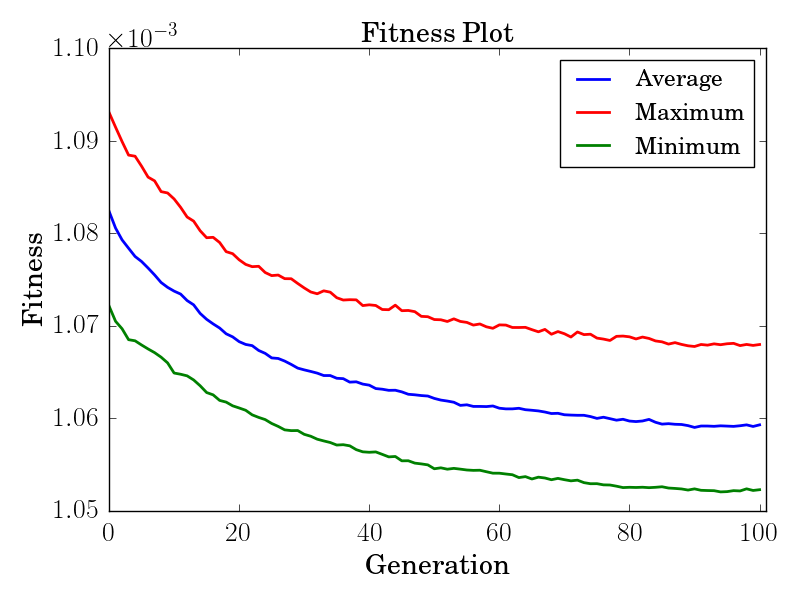
\includegraphics[scale=0.2]{images/"adult selection"/overproduction}
\caption{Overproduction. The newly generated child population consist of twice as many individuals as there are room for in the adult population. Therefore, only the fittest individuals from the large child population grow up into adults.}
\label{figure:overproduction}
\end{center}
\end{figure}



\subsection{Parent Selection}\label{subsection:parent selection}
Parent selection is the process of deciding which adults become parents for the next child generation. When choosing parent selection method there are a few concerns that needs to be addressed. First, it is important that parents with good genes, i.e. lower fitness, gets their genes transferred to the next generation. However, it is also important to keep diversity in the population so that one does not end up with a sub-optimal solution; a local maximum. Two parent selection methods are implemented for the genetic algorithm for this thesis: Tournament selection and roulette wheel selection. \\

\noindent In tournament selection, a given number of individuals are drawn randomly from the population. The number of individuals drawn is decided by the variable \textit{tournament size}. These individuals compete in a tournament for one spot in the parent pool. The individual with best, i.e. lowest fitness, is  selected as a parent. These tournaments continue until the adult pool is full. Figure \ref{figure:tournament selection} shows how tournament selection works. As can be seen in the figure, three individuals are drawn randomly from the adult pool, meaning that the tournament size in this example is 3. The best individual, the individual with fitness 4 is the tournament winner and is allowed to enter the adult pool. In order to maintain diversity in the population there is a small probability that parents are selected randomly from the adult pool instead of with tournament selection. This probability is called \textit{epsilon} and makes sure that a small percent of the parents that might not currently be best are not killed of right away. Different values of the \textit{tournament size} variable needs to be tested in order to find the settings that allow the algorithm to explore different solutions, but that also prioritize the best solutions. In chapter \ref{chapter:results}, results obtained for different values of \textit{tournament size} and \textit{epsilon} are compared. \\


\begin{figure}[h!]
\begin{center}
\includegraphics[scale=0.2]{images/"parent selection"/"tournament selection"}
\caption{Tournament selection. Three individuals with fitness 9, 4 and 6 respectively, are selected randomly from the adult population. The individuals with best fitness, fitness 4, is the tournament winner and is selected into the parent pool.}
\label{figure:tournament selection}
\end{center}
\end{figure}


\noindent Roulette wheel selection assigns a probability of being chosen as parent to each individual proportional to its fitness. Individuals with better fitness will therefore have a higher probability of beings selected into the parent pool. Figure \ref{figure:roulette wheel selection} shows how roulette wheel selection works. The roulette wheel on the left shows the probability for each of the four individuals being selected. Since individual$_4$ has the best fitness, it has a larger probability of being selected than the others. \\


\begin{figure}[h!]
\begin{center}
\includegraphics[scale=0.5]{images/"parent selection"/"roulette wheel selection"}
\caption{Roulette wheel selection. The roulette wheel is shown to the left, the four individuals to the right. Individual$_4$ has a four times better fitness than individual$_2$ and therefore has a four times larger probability of being selected.}
\label{figure:roulette wheel selection}
\end{center}
\end{figure}


\subsection{Genetic Operations}\label{subsection:genetic operations}
This subsection gives an overview over the genetic operations used to produce the next child generation. Three crossover methods, elitism and four mutation methods are implemented and will be presented. 


\subsubsection{Crossover and Elitism}
Crossover is the recombination method utilized by the genetic algorithm to perform sexual reproduction. A crossover operation produced two children by recombining genes of two parent individuals. The genetic algorithm implemented for this thesis has three crossover methods to chose from: Single point crossover, two point crossover and uniform crossover \citep{Magalhaes-Mendes}. These are all presented in figure \ref{figure:crossover methods}. As shown in figure \ref{figure:single point crossover}, single point crossover uses randomly generated position, called the crossover point, to perform recombination. All genes from the first parent prior to the crossover point are copied to the first child, and all genes after the crossover point are copied to the second child, and all genes from the second parent prior to the crossover point is copied to the second child, and all genes after the crossover point is copied to the first child. Two point crossover is similar to single point crossover, except that it uses to crossover points instead of one. This is shown in figure \ref{figure:two point crossover}. In uniform crossover, there is a fifty percent probability that each gene will be drawn from each parent as shown in figure \ref{figure:uniform crossover}. This crossover method mix up the parent genes more that the two others, therefore more gene patterns will be lost using this method. Even though crossover is the main recombination method it is not used for creating every child individual. Some child individuals are copies of their parents with potential small mutation in their genes. The number of individuals created using crossover is decided by the crossover rate. Crossover rates are usually kept pretty high since the goal is to evolve new and better solutions, however test runs presented in chapter \ref{chapter:results} do confirm that it is good to let a percentage of the children be produced without crossover. \\


\begin{figure}[h!]
    \centering
    \begin{subfigure}[b]{0.3\textwidth}
        \includegraphics[width=\textwidth]{images/crossover/"Single point crossover"}
        \caption{}
        \label{figure:single point crossover}
    \end{subfigure}
    ~ 
    \begin{subfigure}[b]{0.3\textwidth}
        \includegraphics[width=\textwidth]{images/crossover/"Two point crossover"}
        \caption{}
        \label{figure:two point crossover}
    \end{subfigure}
    ~
    \begin{subfigure}[b]{0.3\textwidth}
        \includegraphics[width=\textwidth]{images/crossover/"Uniform crossover"}
        \caption{}
        \label{figure:uniform crossover}
    \end{subfigure}
    \caption{Crossover methods: (a) Single point crossover, (b) two point crossover, and (c) uniform crossover.}
    \label{figure:crossover methods}
\end{figure}


\noindent A method used to make sure that the best individuals in the population does not get killed of by accident is called \textit{elitism}. Elitism simply takes the best individual(s) from the parent population and copies it(them) directly into the new child population without performing any genetic operations on it(them). Elitism is commonly used with genetic algorithm and will be used in this thesis. 


\subsubsection{Mutation}
Although crossover is a powerful genetic operator that makes sure that child individuals to inherit genes from the best parent individuals, it is not enough by itself. Without any way to mutate genes, one can end up with a population where every individual has the same gene value in the same position, this means that no recombination method will be able to change the value of that gene. Mutation is the operation used by the genetic algorithm to make sure that the population do not get sterile. In nature, genes can be mutated in numerous ways. In this thesis, three mutation methods are implemented to mimic the mutations methods that can happen in genes \citep{Soni}, these are called: Flip mutation, interchanging mutation, and inversion mutation. Flip mutation, shown in figure \ref{figure:flip mutation}, is the most common mutation method used in genetic algorithms. As it's name implies, flip mutation works by flipping the value of bits in the genotype. Usually, mutation rates are low since one do not want mutation to make to many changes to the good genes inherited from parent individuals, but simply introduce some diversity. Therefore, only a couple of bits are mutated in each genotype each generation. Interchange mutation and inversion mutation are rarely used in genetic algorithms, however they are included in this thesis to introduce even more diversity in the population and hopefully help the genetic search finding even better solutions. They both introduce more change than flip mutation, and will be assigned rates even lower than the mutation rate for flip mutation. Figure \ref{figure:interchange mutation} and \ref{figure:inversion mutation} shows interchange- and inversion mutation respectively. Interchange mutation works by by picking two random genes and interchange their values, while inversion mutation works by picking two random positions and invert each gene between those positions. 


\begin{figure}[h!]
    \centering
    \begin{subfigure}[b]{0.3\textwidth}
        \includegraphics[width=\textwidth]{images/mutation/"flip mutation"}
        \caption{}
        \label{figure:flip mutation}
    \end{subfigure}
    ~ 
    \begin{subfigure}[b]{0.3\textwidth}
        \includegraphics[width=\textwidth]{images/mutation/"interchanging mutation"}
        \caption{}
        \label{figure:interchange mutation}
    \end{subfigure}
    ~
    \begin{subfigure}[b]{0.3\textwidth}
        \includegraphics[width=\textwidth]{images/mutation/"inversion mutation"}
        \caption{}
        \label{figure:inversion mutation}
    \end{subfigure}
    \caption{Mutation methods: (a) Single point crossover, (b) two point crossover, and (c) uniform crossover.}
    \label{figure:mutation methods}
\end{figure}


\subsection{Wind-, Wake- and Power Model}\label{subsection:wind-, wake- and power model}
The evaluation class uses the same wake-, wind- and power model as \cite{Kusiak}. The wake model used is the classical Jensen model \citep{Jensen}, which is used in almost every study of the wind farm layout optimization problem, as can be seen in table \ref{table:overview}. \\

\noindent Wind distribution is modeled using the Weibull distribution, a continuous probability distribution shown to model wind distribution quite well \citep{Justus}. The probability density function is shown in equation \ref{equation:Weibull}


\begin{equation}
f(x; c, k)  = 
\begin{cases}
\frac{k}{c} \left( \frac{x}{c} \right)^{k-1} e^{- \left( \frac{x}{c} \right)^k } & \text{if} \hspace{1mm} x \geq 0 \\
0                                                                                                                      & \text{if} \hspace{1mm}     x < 0
\end{cases}
\label{equation:Weibull}
\end{equation}


\noindent where $k$ is called the shape parameter and $c$ is the scale parameter, and $k, c > 0$. In most of the wind scenarios provided by GECCO 2016, $k \approx 2$, this is shown empirically to be a good value for wind speed distribution \citep{Justus}. On the other hand, the shape parameter vary for each wind direction. Figure \ref{figure:weibull distribution} shows the Weibull distribution plotted for $k = 2$ and for different values of $c$. \\


\begin{figure}[h!]
\begin{center}
\includegraphics[scale=0.4]{images/"Weibull"}
\caption{The Weibull distribution plotted for $k = 2$ for different values of the scale parameter $c$.}
\label{figure:weibull distribution}
\end{center}
\end{figure}

\noindent The wind scenarios used in this thesis are therefore a specification of the shape- and scale parameters for every wind direction, where wind direction is partitioned into 24 different directions. Twenty wind scenarios are provided by GECCO 2016, 10 which simply specify wind distribution parameters, and 10 that specify wind distribution parameters and locations of obstacles. \\

\noindent The power curve used is also the same as used in \cite{Kusiak}, it is the linear function shown in equation \ref{equation:Power Curv (API)},

\begin{equation}
 f(v) = 
  \begin{cases} 
   0                                  & \text{if }     v < v_{cut-in} \\
   \lambda v + \eta           & \text{if }     v_{cut-in} \leq v \leq v_{rated} \\
   P_{rated}                        & \text{if }     v_{cut-out} > v > v_{rated}. \\
  \end{cases}
  \label{equation:Power Curv (API)}
\end{equation}

\noindent Here $\lambda$ is the slope parameter, $v$ the wind speed, $\eta$ the intercept parameter, $P_{rated}$ is the fixed power output, and $v_{cut-in}$ is the cut-in speed; the minimum speed for which the turbine produces power, and $v_{cut-out}$ is the cut-out speed; the maximum wind speed for which the turbine is kept on. 


\subsection{Fitness Function}\label{subsection:fitness function}
The main task of the evaluation classes is to calculate the fitness of each individual based on the fitness function.  The fitness function to be optimized is provided by GECCO 2016, and is displayed in equation \ref{Objective function}.\\

\begin{small}
\begin{equation}
fitness =  \frac{ \left( c_t \cdot n + c_s \cdot \floor*{\frac{n}{m}} \right) \left( \frac{2}{3} + \frac{1}{3} \cdot e^{-0.00174n^2} \right) + c_{OM} \cdot n}{\left( \frac{1 - (1 + r)^{-y}}{r} \right) } \cdot \frac{1}{8760 \cdot P} + \frac{0.1}{n}
\label{Objective function} 
\end{equation}
\end{small}


\noindent Description and numerical values of all parameters given in equation \ref{Objective function} are displayed in table \ref{Parameters}. As can be seen in this table, the values of $n$, the number of turbines, and $P$, farm energy output, are not given. This is because the number of turbines, together with the turbine positions, are the parameters to be optimized by the genetic algorithm. Farm energy output is the indirect parameter that we are trying to optimize. It is dependent on turbines count, position, wind scenario and so on, and is off course therefore not provided in table \ref{Parameters} either.\\


\begin{table}[h!]
\begin{center}
\caption{Description and value of each parameter used in the objective function provided by GECCO 2015.}
\label{Parameters}
\begin{tabular}{l|l|l}
\textbf{Parameter} & \textbf{Description} & \textbf{Value} \\ 
\hline 
$c_t$ & Turbine cost (usd) & 750 000 \\ 
$c_s$ & Substation cost (usd) & 8 000 000 \\ 
$m$ & Turbines per substation & 30 \\ 
$r$ & Interest rate & 0.03 \\ 
$y$ & Farm lifetime (years) & 20 \\ 
$c_{OM}$ & Yearly operating costs per turbine & 20 000 \\ 
$n$ & Number of turbines &  \\ 
$m$ & Farm energy output &  \\  
\end{tabular} 
\end{center}
\end{table}


\noindent Intuitively, the objective function can be divided into different parts. The first parenthesis in the nominator of the first fraction is the construction cost, while the second parenthesis is the economies of scale and the third part of the nominator is yearly operating costs. The denominator represents the interests. The denominator of the second fraction describes yearly power output, while the number $0.1$ in the nominator of the last fraction is a farm size coefficient. \\


\section{Scenarios}\label{section:scenarios}


\begin{figure}[h!]
\begin{center}
\includegraphics[scale=0.4]{images/obstacles}
\caption{Obstacles are described in the scenarios with its (x, y)-boundaries.}
\label{figure:obstacles}
\end{center}
\end{figure}


GECCO 2016 has provided the contestants with 20 different wind scenarios for which the genetic algorithm can be tested on. Each wind scenario contain shape and scale parameters, k and c respectively, for each wind directions where wind direction is partitioned into slots that cover an 15 degree angle each, so that there are 24 different wind directions. Unavailable areas are described in the scenario by the parameters \textit{x$_{min}$, x$_{max}$, y$_{min}$} and \textit{y$_{max}$} as shown in figure \ref{figure:obstacles}. In the figure, two obstacles are described giving their (x, y)-boundaries. The red lines gives the boundaries of obstacle 1 and the blue lines gives the boundaries of obstacle 2. The yellow area in the middle of the lines shows the illegal areas. Each wind scenario also contain values for the constants ''width'', ''height'', ''number of turbines'' and ''wake free energy''. The scenarios are read from file at the beginning of each run of the genetic algorithm. 


\section{Population Distributed Genetic Algorithms: Implementation Details}\label{section:population distributed gas implementation details}


Now that the reader is familiar with how individuals are represented, which selection mechanisms and genetic operators that are implemented, how fitness is calculated, and how the scenarios look, it is time to go into details of how the population distributed genetic algorithms are implemented. Although the population distributed genetic algorithms were introduced in chapter \ref{chapter:background}, the details of how each step in figure \ref{figure:genetic algorithm steps} are implemented for each model was not given. Therefore, this section contains a detailed description of how the population distributed genetic algorithms are implemented. \\


\noindent One decision that can be mentioned here, because it applies to all the models below, is whether the three population distributed genetic algorithms are heterogeneous or homogeneous. In an homogeneous environment, the same rules apply to the entire model. This means that the same adult- and parent selection mechanisms, the same genetic operators and the same fitness function is used for the entire model, it is not different for different Islands (Island model), threads (Pool model) or areas (Cellular model). Even thought it would be very interesting to implement heterogeneous models, it is not done in this thesis. The reason behind this decision is that it is best to let the same rules apply to every part of every model when different models are compared.\\


\subsection{The Island Model}


\noindent The Island model works as follows: A population of individuals are partitioned into sub populations which are distributed onto different Islands. An Island can be connected to one or more Islands and individuals on one Island can migrate to other Islands following one of the migration routes. Table \ref{table:parameter description island model} gives an description of the Island model parameters. For a number of generations, decided by the variable \textit{migration interval}, the population on one Island follow the steps of the simple genetic algorithm from figure \ref{figure:genetic algorithm steps}. However, when the population has evolved for \textit{migration interval} generations some individuals from one Island can migrate to another Island. These two steps continue until the total number of generations reaches some predefined value.\\


\noindent As mentioned in chapter \ref{chapter:background} the Island model can be implemented with either synchronized or asynchronized migration. Synchronized migration means that migration is performed at the same generation for all Island, and asynchronized migration means that migration can be performed whenever an Island is ready. In this thesis, the Island model is implemented with synchronous migration in order to not over-complicate the migration function.\\


\begin{table}[h!]
    \centering
    \caption{Island model parameter description.}
    \label{table:parameter description island model}
        \begin{tabular}{l|l}
         \textbf{Parameter} & \textbf{Description}  \\
         \hline
         Deme size  & Number of individuals on each Island (deme) \\
         Deme count & Number of Islands (demes) \\
         Migration rate & Number of individuals that migrate \\
         Migration interval & Number of generations between migration. \\
         Number of migrations & Total number of times migration is performed. \\
         Topology & Circular
    \end{tabular}
\end{table}


\noindent As mentioned, migration means that individuals migrates to another Island. In this thesis, migration from one Island to another means that the best individuals in Island \textit{i} is copied onto Island \textit{j} to replace the individuals with lowest fitness on Island \textit{j}. In other words, migration does not mean that the best individuals in Island \textit{i} leaves that Island, but that copies of them replace the individuals with worst fitness on Island \textit{j}. The number of individuals that migrate is decided by the parameter \textit{migration rate}.\\


\noindent As described in table \ref{table:parameter description island model} the topology implemented in this thesis is circular. This can be seen in figure \ref{figure:topology island model} where the legal migration routes are indicated by arrows. Since individuals are only allowed to migration in one direction with this topology it will take time (many generations) for the individual on the upper-right Island to travel to the upper-left Island since they have to go through both Islands on the bottom. This means that different parts of the solution space can be explored on different Island before individuals from one Island take over the entire population.


\begin{figure}
    \begin{center}
        \includegraphics[scale=0.5]{"island model topology"}
        \caption{Island model topology.}
        \label{figure:topology island model}
    \end{center}
\end{figure}


\subsection{Pool Model}


\noindent In the Pool model, the individuals are distributed in a resource pool. The resource pool is partitioned into equal size partitions so that one thread is responsible for one partition. Each thread selects \textit{x} individuals from the entire population, where \textit{x} is equal to the total population size divided by the total number of threads. Next, each thread generates a child pool by performing genetic operations on the selected individuals. After the new child pool is generated, each child individual is compared against the individual in the resource pool currently occupying its designated position. If the fitness of the new individuals is better than the fitness of the old individual the new child individual overwrites the old individuals. This is illustrated in figure \ref{figure:pool model update function}. As can be seen in the figure thread \textit{i} overwrites the individuals in positions 1, 3 and 4 in the partition it is responsible for.\\


\begin{figure}[h!]
\begin{center}
\includegraphics[scale=0.5]{images/"pool model update function"}
\caption{Pool model updating function. For each generation, each thread updates its region if the new individuals are better than the individuals currently occupying the position.}
\label{figure:pool model update function}
\end{center}
\end{figure}


\noindent The pool model is asynchronous by nature. The threads operate unaware of each other. Since each thread only writes to its own positions in the resource pool, it is not a problem that the threads work independently without any form of synchronization. By implementing the Pool model this way some parts of the resource pool might have better fitness that others because they have evolved for more generations than other parts. This property ensures that different parts of the search space is explored in different regions of the resource pool. \\


\noindent As mentioned above, parent individuals are selected from the entire resource pool. However, parents are not picked completely at random. For each parent selected a group of potential parents are selected at random from the resource pool, and these individuals compete for the spot in the parent pool by tournament selection. This guides the evolution in the right direction. Picking individuals at random might also work for this model since the new individuals are only written back if they are better than the previous individuals, however, this would make evolution extremely slow, and it would not make sense from an evolutionary point of view because the fittest individuals are not prioritized.


\subsection{Cellular Model}


\noindent The Cellular model distributes the population in a square grid. Each individual has its own cell which corresponds to an (x, y)-position. For each generation, each cell is updated. Each cell in the grid is updated by selecting parent individuals that are close to the given cell, perform genetic operations on those parents and write the newly generated individual back to the cell.\\


\noindent As mentioned in the background, the cells in the Cellular model could either be updated in a synchronous fashion or an asynchronous fashion. In this thesis the updating is synchronous, meaning that the cells are updated simultaneously.\\


\noindent The topology used in this thesis is a square topology, as shown in figure \ref{figure:cellular model topology}. Only individuals within the square can be selected as parents for the middle cell. Parent selection are performed by tournament selection within the square. By distributing individuals in a grid different parts of the grid will explore different regions of the search space.\\


\begin{figure}
\centering
\includegraphics[scale=0.5]{"images/cellular model topology"}
\caption{Cellular model topology. Only individuals within the marked square are allowed to become parents for the middle cell.}
\label{figure:cellular model topology}
\end{figure}


\section{Motivation behind Implementing the Genetic Algorithm from Scratch}\label{section:motivation}
Even though GECCO	 2016 has provided each contestant with an API which could be used directly, or improved upon and used in the competition, the decision to implement the genetic algorithm from scratch was made. Even though this decision lead to more work for the author, several arguments supported the decision. First of all, even though the provided API was implemented in Java, it was not very object oriented nor was it modular, something that made it very difficult to add new features to the code without having to do major changes. In addition, the provided genetic algorithm was extremely simple with no room for making any decisions about which method to use for any of the steps in figure \ref{figure:genetic algorithm steps}. Other problems such as hard-coded variables and too long methods made it very difficult to make changes and add new features. \\

\noindent The new genetic algorithm is implemented so that new selection methods can be added by simply implementing the AdultSelection- or ParentSelection interface, and new crossover methods can be added by extending the Crossover class. This makes the program much more flexible, if one wish to try something new. No variables are hard-coded in the new program, but taken as parameters to the GeneticAlgorithm constructor, leaving no room for making errors. The major improvement, and most important motivation behind the decisions of implementing the genetic algorithm from scratch is that it gives the author total control over every aspect of the code, and it was very important with modular code when the population distributed genetic algorithms were implemented.\\

\noindent In summary, this chapter contains the implementation detail of the genetic algorithm implemented for this thesis. Now that the reader is familiar with how the different genetic algorithm models are implemented it is time to take a closer look at the results obtained in this thesis. \\
\chapter{Results and Discussion}\label{chapter:results}
This chapter includes presentation and analysis of the results obtained in this thesis. Section \ref{section:parameter settings} presents results from testing different parameter settings for the genetic algorithm, and briefly discusses each results. Section \ref{section:results} presents the main results obtained when running the different population distributed genetic algorithms. Section \ref{section:discussion} contains a discussion and comparison of the results obtained in section \ref{section:results}.


\section{Parameter settings}\label{section:parameter settings}
Parameter settings are crucial for obtaining good results with the genetic algorithm. In order to find the right settings, simulations were run to find the best adult selection method, parent selection method, crossover method, crossover rate and mutation rate for the given problem. Even though it would take much shorter time and less effort to test these settings on a toy problem such as One Max, the decision was made to test them on the real problem. The reason behind this decision is that different settings might work better on different problems and the nature of the wind farm layout optimization problem is unique because of the importance of the wind turbine positions relative to each other. It is important to note that even though effort was made to find good settings for the genetic algorithm,  it is impossible to obtain the optimal ones. Just imagine trying the test every single value for the continuous parameter crossover rate against every possible value of each of the other settings, just that would be impossible! Therefore, the values that are tested for each parameter setting is largely tested against values that are based on the authors previous experience with genetic algorithm and values close to those.\\

\begin{table}
\centering
\caption{Values kept fixed while one by one was changed in order to find the best settings for the wind farm layout optimization problem.}
\label{table:fixed settings}
\begin{tabular}{l|l}
\textbf{Parameter} & \textbf{Value} \\ 
\hline 
Wind scenario & 00.xml \\ 
Evaluator & KusiakLayoutEvaluator \\ 
Population size & 100 \\  
Generations & 100 \\ 
Elitism & true \\  
Flip mutation rate & 0.01 \\ 
Inversion mutation rate & 0.0 \\ 
Interchange mutation rate & 0.0 \\ 
Parent selection & Tournament selection \\ 
Tournament size & 5 \\ 
Epsilon & 0.0 \\  
Crossover method & Uniform crossover \\ 
Crossover rate & 0.9 \\ 
\end{tabular} 
\end{table}

\noindent For each simulation one of the parameters were tested while the others were kept fixed as shown in table \ref{table:fixed settings}. As can be seen in this table, other settings such as wind scenario, population size, number of generations, whether elitism should be used and mutation rate for interchange mutation and inversion mutation could also be tested, but since evaluation of each farm takes a lot of time, even on an 8 core computer running in parallel, simulations are not run to set these values. These settings are set using the authors previous experience and educated guessing. Testing different parameters on a single wind scenario might lead to values that are tailored for the given scenario and that are not as well suited for some of the others. However, there is no time to test each value for every single wind scenario, and this should not make that much of a difference. Population size is a value that influence the performance of the genetic algorithm largely. Greater population size often leads to better performance since more solutions increase the probability of finding the global optimal solution. The population size was set to 100 for two reasons. First of all, a population size of 100 is large enough so that many different solutions are explored. Second when the population size is kept at 100, the adult selection method ''Overproduction'' will produce twice as many children, so that 200 individuals has to be evaluated for each generation something that will double the evaluation time, the step that already is the bottleneck of the algorithm. The number of generations was kept at 100 for each run, evaluating each population for 100 generations takes time and it the main reason why the algorithm were not run for more generations, however, as can be seen on the graphs in the sections below the fitness looks like it is starting to flat out after a 100 generations indicating that a 100 generations are sufficient for the purpose of setting the parameter values. Elitism was set to true for every run without testing, meaning that the best individual of each generation will survive. This decision is based on the authors previous experience with genetic algorithm where experiments has shown that elitism leads to better results because the best individual is not lost due to coincidences. Different mutation methods were implemented for the genetic algorithm, but only the flip mutation rate was tested to find the best value. Usually, flip mutation is the only mutation method used with genetic algorithms and it is therefore also used as the main for of mutation in this thesis. Inversion mutation and interchange mutation are implemented, but they will only happen seldom to introduce more randomness to the algorithm. In the main simulations, they will be assigned extremely low probabilities so that their occurrence is so rare that they will introduce too much randomness, but hopefully make occasional ''jumps'' to different solutions spaces so that the algorithm do not get completely stuck in a local optimal solution. 


\subsection{Adult Selection}
Figure \ref{figure:adult selection methods} shows the results of running the genetic algorithm with the different adult selection methods. Figure \ref{figure:full generational replacement}, \ref{figure:generational mixing}, and \ref{figure:overproduction} shows the results for full generational replacement, generational mixing and overproduction respectively. As can be seen in the figures, full generational replacement ends up with an average best fitness of \textcolor{red}{average of best fitness}, generational mixing with an average best fitness of \textcolor{red}{average of best fitness}, and overproduction with an average best fitness of \textcolor{red}{average of best fitness}. These results are as expected. Note that generational mixing could never do worse than full generational replacement. If the results of reproduction leads to a population of individuals with strictly better fitness, generational mixing will replace the entire previous generation with the new one, as full generational replacement. However, if the new generation produces individuals with worse fitness than some of the individuals in the previous generation these old individuals will be kept instead, making sure that the new population has equal or better fitness than the previous one. Overproduction does not provide the same ''newer worst'' \textcolor{red}{Check word!} guarantee, however, as shown in figure \ref{figure:overproduction} it still outperforms generational mixing. Even though overproduction wipes out the entire previous population, it generates twice as many children at the reproduction step so its probability of getting it right is doubled. 


\begin{figure}[h!]
    \centering
    \begin{subfigure}[b]{0.31\textwidth}
        \includegraphics[width=\textwidth]{images/plots/"adult selection"/"full generational replacement"}
        \caption{}
        \hfill
        \label{plot:full generational replacement}
    \end{subfigure}
    ~
    \begin{subfigure}[b]{0.31\textwidth}
        \includegraphics[width=\textwidth]{images/plots/"adult selection"/"generational mixing"}
        \caption{}
        \hfill
        \label{plot:generational mixing}
    \end{subfigure}
    ~
    \begin{subfigure}[b]{0.31\textwidth}
        \includegraphics[width=\textwidth]{images/plots/"adult selection"/"overproduction"}
        \caption{}
        \hfill
        \label{plot:overproduction}
    \end{subfigure}
    \caption{Adult selection methods: (a) Full generational replacement, (b) generational mixing and (c) overproduction averaged over 10 runs.}
    \label{plot:adult selection methods}
\end{figure}


\subsection{Parent Selection}


\begin{figure}[h!]
    \centering
    \begin{subfigure}[b]{0.31\textwidth}
        \includegraphics[width=\textwidth]{images/plots/"parent selection"/"roulette wheel"}
        \caption{}
        \hfill
        \label{plot:roulette wheel}
    \end{subfigure}
    ~
    \begin{subfigure}[b]{0.31\textwidth}
        \includegraphics[width=\textwidth]{images/plots/"parent selection"/"tournament size 5"}
        \caption{}
        \hfill
        \label{plot:tournament size 5}
    \end{subfigure}
    ~
       \begin{subfigure}[b]{0.31\textwidth}
        \includegraphics[width=\textwidth]{images/plots/"parent selection"/"tournament size 10"}
        \caption{}
        \hfill
        \label{plot:tournament size 10}
    \end{subfigure}
    ~
       \begin{subfigure}[b]{0.31\textwidth}
        \includegraphics[width=\textwidth]{images/plots/"parent selection"/"tournament size 15"}
        \caption{}
        \hfill
        \label{plot:tournament size 15}
    \end{subfigure}
    ~
       \begin{subfigure}[b]{0.31\textwidth}
        \includegraphics[width=\textwidth]{images/plots/"parent selection"/"tournament size 20"}
        \caption{}
        \hfill
        \label{plot:tournament size 20}
    \end{subfigure}
    ~
    \begin{subfigure}[b]{0.31\textwidth}
        \includegraphics[width=\textwidth]{images/plots/"parent selection"/"tournament size 25"}
        \caption{}
        \hfill
        \label{plot:tournament size 25}
    \end{subfigure}
    \caption{Parent selection methods: (a) Roulette wheel, (b) Tournament selection averaged over 10 runs, tournament size 5 (c) tournament selection, tournament size 10, (d) tournament selection, tournament size 15, (e) tournament selection, tournaments size 20, and (f) tournament selection, tournament size 25.}
    \label{plot:parent selection}
\end{figure}


\begin{figure}[h!]
    \centering
    \begin{subfigure}[b]{0.31\textwidth}
        \includegraphics[width=\textwidth]{images/plots/epsilon/"tournament size 20"/"epsilon 0,05"}
        \caption{}
        \hfill
        \label{plot:single point crossover}
    \end{subfigure}
    ~
    \begin{subfigure}[b]{0.31\textwidth}
        \includegraphics[width=\textwidth]{images/plots/epsilon/"tournament size 20"/"epsilon 0,10"}
        \caption{}
        \hfill
        \label{plot:two point crossover}
    \end{subfigure}
    ~
    \begin{subfigure}[b]{0.31\textwidth}
        \includegraphics[width=\textwidth]{images/plots/epsilon/"tournament size 20"/"epsilon 0,15"}
        \caption{}
        \hfill
        \label{plot:uniform crossover}
    \end{subfigure}
    \caption{Different epsilon values averaged 10 runs when tournament size was kept at 20: (a) Epsilon 0.05, (b) epsilon 0.10 and (c) epsilon 0.15.}
    \label{plot:crossover methods}
\end{figure}


\subsection{Crossover Methods}
Figure \ref{figure:crossover methods} displays the results from running the genetic algorithm with single point crossover, two point crossover and uniform crossover showed in sub figures \ref{figure:single point crossover}, \ref{figure:two point crossover} and \ref{figure:uniform crossover} respectively. As can be seen in the figure, there is no crossover method that stands out, but end up with similar fitness. Single point crossover ends up with an averaged best fitness of \textcolor{red}{averaged best fitness}, two point crossover ends up with an averaged fitness of \textcolor{red}{averaged best fitness} and uniform crossover ends up with an averaged fitness of \textcolor{red}{averaged best fitness}. Intuitively, one would expect uniform crossover to perform worse than the others because it mixes up the relative positions between the wind turbines more than single- and two point crossover, however it actually obtains slightly better fitness. Even though it obtains slightly better fitness this could be a coincidence since the different is so small, and the simulations are only averaged over ten runs. \textcolor{red}{Explanation behind the results, talk to Keith. Stupid paragraph change everything!}


\begin{figure}[h!]
    \centering
    \begin{subfigure}[b]{0.31\textwidth}
        \includegraphics[width=\textwidth]{images/plots/"crossover method"/"single point crossover"}
        \caption{}
        \hfill
        \label{plot:single point crossover}
    \end{subfigure}
    ~
    \begin{subfigure}[b]{0.31\textwidth}
        \includegraphics[width=\textwidth]{images/plots/"crossover method"/"two point crossover"}
        \caption{}
        \hfill
        \label{plot:two point crossover}
    \end{subfigure}
    ~
    \begin{subfigure}[b]{0.31\textwidth}
        \includegraphics[width=\textwidth]{images/plots/"crossover method"/"uniform crossover"}
        \caption{}
        \hfill
        \label{plot:uniform crossover}
    \end{subfigure}
    \caption{Crossover methods averaged over 10 runs: (a) Single point crossover, (b) two point crossover and (c) uniform crossover.}
    \label{plot:crossover methods}
\end{figure}


\subsection{Crossover Rate}


\begin{figure}[h!]
    \centering
    \begin{subfigure}[b]{0.31\textwidth}
        \includegraphics[width=\textwidth]{images/plots/"crossover rate"/"crossover rate 0,0"}
        \caption{}
        \hfill
        \label{plot:crossover rate 0.0}
    \end{subfigure}
    ~
    \begin{subfigure}[b]{0.31\textwidth}
        \includegraphics[width=\textwidth]{images/plots/"crossover rate"/"crossover rate 0,2"}
        \caption{}
        \hfill
        \label{plot:two point crossover}
    \end{subfigure}
    ~
       \begin{subfigure}[b]{0.31\textwidth}
        \includegraphics[width=\textwidth]{images/plots/"crossover rate"/"crossover rate 0,4"}
        \caption{}
        \hfill
        \label{plot:two point crossover}
    \end{subfigure}
    ~
       \begin{subfigure}[b]{0.31\textwidth}
        \includegraphics[width=\textwidth]{images/plots/"crossover rate"/"crossover rate 0,6"}
        \caption{}
        \hfill
        \label{plot:two point crossover}
    \end{subfigure}
    ~
       \begin{subfigure}[b]{0.31\textwidth}
        \includegraphics[width=\textwidth]{images/plots/"crossover rate"/"crossover rate 0,8"}
        \caption{}
        \hfill
        \label{plot:two point crossover}
    \end{subfigure}
    ~
    \begin{subfigure}[b]{0.31\textwidth}
        \includegraphics[width=\textwidth]{images/plots/"crossover rate"/"crossover rate 1,0"}
        \caption{}
        \hfill
        \label{plot:uniform crossover}
    \end{subfigure}
    \caption{Crossover rates: (a) Crossover rate 0.0, (b) crossover rate 0.2, (c) crossover rate 0.4, (d) crossover rate 0.6, (e) crossover rate 0.8, and (f) crossover rate 1.0.}
    \label{plot:crossover methods}
\end{figure}


\subsection{Mutation Rate}


\begin{figure}[h!]
    \centering
      \begin{subfigure}[b]{0.31\textwidth}
        \includegraphics[width=\textwidth]{images/plots/"mutation rate"/"mutation rate 0,0001"}
        \caption{}
        \hfill
        \label{plot:single point crossover}
    \end{subfigure}
    ~
      \begin{subfigure}[b]{0.31\textwidth}
        \includegraphics[width=\textwidth]{images/plots/"mutation rate"/"mutation rate 0,0005"}
        \caption{}
        \hfill
        \label{plot:single point crossover}
    \end{subfigure}
    ~
    \begin{subfigure}[b]{0.31\textwidth}
        \includegraphics[width=\textwidth]{images/plots/"mutation rate"/"mutation rate 0,001"}
        \caption{}
        \hfill
        \label{plot:single point crossover}
    \end{subfigure}
    ~
    \begin{subfigure}[b]{0.31\textwidth}
        \includegraphics[width=\textwidth]{images/plots/"mutation rate"/"mutation rate 0,005"}
        \caption{}
        \hfill
        \label{plot:two point crossover}
    \end{subfigure}
    ~
    \begin{subfigure}[b]{0.31\textwidth}
        \includegraphics[width=\textwidth]{images/plots/"mutation rate"/"mutation rate 0,01"}
        \caption{}
        \hfill
        \label{plot:uniform crossover}
    \end{subfigure}
    \caption{Mutation rates: (a) Mutation rate 0.0001, (b) mutation rate 0.0005 and (c) mutation rate 0.001, (d) mutation rate 0.005 and (e) mutation rate 0.01s.}
    \label{plot:crossover methods}
\end{figure}


\section{Results}\label{section:results}
\noindent In table \ref{table:final parameter settings master slave model} the parameter values used when running the master slave model is shown. The crossover method, crossover rate, mutation rate, adult selection mechanism, parent selection mechanism and parent selection parameters are those that proved to work best for the wind farm layout optimization problem as shown in the previous section. The population size was set to 100 and the number of generations to 200. A population size of 100 is quite small, but since overproduction is the selected adult selection method a population size of 100 leads to evaluation of 200 individuals each generation. Since evaluation is the bottle neck, by far, for wind farm layout optimization a larger population size would not be possible to evaluate for 200 generations. A possibility could be to pick a larger population size and a smaller number of generations, but since the objective of this thesis is to explore population distributed genetic algorithms a large number of generations is crucial since population distributed genetic algorithms need more time to find good solutions since they explore different search spaces. \\


\begin{table}
\centering
\caption{Parameter values used for the master slave model.}
\label{table:final parameter settings master slave model}
\begin{tabular}{l|l}
\textbf{Parameter} & \textbf{Value} \\ 
\hline 
Population size & 100 \\  
Generations & 200 \\ 
Crossover method & Single point crossover \\ 
Crossover rate & 0.9 \\ 
Elitism & True \\ 
Flip mutation rate & 0.001 \\ 
Inversion mutation rate & 0.000001 \\ 
Interchange mutation rate & 0.000001 \\ 
Adult selection mechanism & Overproduction \\ 
Parent selection mechanism & Tournament selection \\ 
Tournament size & 20\% of population size\\ 
Epsilon & 0.1 \\ 
\end{tabular} 
\end{table}


\noindent Table \ref{table:final parameter settings island model} shows the parameters from the Island model that differs from the ones in table \ref{table:final parameter settings master slave model}. The deme size, number of individuals on each Island, is set to 26 resulting in a total population size of 104, not 100 as in table \ref{table:final parameter settings master slave model}. The reason behind this is that the implementation requires a population size of even numbers. The deme count, number of Islands, is set to four and the topology is circular as shown in figure \textcolor{red}{(Make topology figure)}. In order to let the populations on the different Islands explore different search spaces 20 generations are run before migration is performed. Migration is performed 10 times so that the total number of generations becomes 200 as for the master slave model. \\


\begin{table}
\centering
\caption{Parameter values used for the Island model.}
\label{table:final parameter settings island model}
\begin{tabular}{l|l}
\textbf{Parameter} & \textbf{Value} \\ 
\hline 
Deme size & 26 \\
Total population size & 104 \\  
Deme count & 4 \\
Migration rate & 2 \\
Number of migrations & 10 \\ 
Migration interval & 20 \\
Topology & Circular  \textcolor{red}{reference figure} \\
\end{tabular}
\end{table}


\begin{figure}
\centering
\includegraphics[scale=0.5]{"images/island model topology"}
\caption{Island model topology. Individuals are only allowed to migrate in the directions indicated by the arrows.}
\label{figure:islandsland Modell titeritroexThThe hets difsH." model topology}
\end{figure}


\noindent As can be seen in table \ref{table:final parameter settings pool model} the cellular model has a population size of 225. At a first glance this might seem like an odd decision since the models above has a population size of about 100 individuals, but the reason is simple. Since overproduction is the adult selection mechanism used for the models above 200 individuals are evaluated for each generation, however, overproduction is not used with the cellular model because each individual has its own position in the grid so that growing and shrinking the population at different stages of the genetic algorithm does not make sense. By using a population size of about 200 the cellular model get approximately the same processor time as the algorithms above, and therefore the comparison becomes more fair than with a population size of 100. The reason why the population size is 225 and not 200 is because a quadratic grid is used to distribute the production and 225 is equal to 15$^{2}$. As can be seen in figure \ref{figure:cellular model topology}, the topology used is a simple square containing nine individuals, the individual in the middle square can only be replaced by individuals generated by recombining individuals within the square grid. The decision to make the neighborhood this small is that it will give different solutions the opportunity to dominate different areas of the grid, giving the algorithm the time to explore different solution spaces.\\


\begin{table}
\centering
\caption{Parameter values used for the cellular model.}
\label{table:final parameter settings cellular model}
\begin{tabular}{l|l}
\textbf{Parameter} & \textbf{Value} \\ 
\hline 
Population size & 225 \\
Topology & \textcolor{red}{reference figure} \\  
\end{tabular}
\end{table}


\begin{figure}
\centering
\includegraphics[scale=0.5]{"images/cellular model topology"}
\caption{Cellular model topology. Only individuals within the marked square are allowed to become parents for the middle cell.}
\label{figure:cellular model topology}
\end{figure}


\noindent Table \ref{table:final parameter settings pool model} shows the parameter values used by the pool model that differs from those in table \ref{table:final parameter settings master slave model}. As for the cellular model, the population size is set to 200 so that 200 evaluations are performed for each of the 200 generations. Since child generation for the pool model consist of producing one individual for each position which the given thread is responsible for it makes no sense to use overproduction, therefore a population size of 200 gives the algorithm as much processor time as the three others.\\


\begin{table}
\centering
\caption{Parameter values used for the pool model.}
\label{table:final parameter settings pool model}
\begin{tabular}{l|l}
\textbf{Parameter} & \textbf{Value} \\ 
\hline 
Population size & 200 \\  
Number of workers & 4 \\ 
\end{tabular}
\end{table}


\noindent \textcolor{red}{Write about evaluation parameters. Fix graphs and display results.}


\begin{figure}[h!]
    \centering
      \begin{subfigure}[b]{0.31\textwidth}
        \includegraphics[width=\textwidth]{images/plots/Plots/"scenario 00"/"best"}
        \caption{Fitness}
        \hfill
        \label{plot:fitness plot scenario 00}
    \end{subfigure}
    ~
      \begin{subfigure}[b]{0.31\textwidth}
        \includegraphics[width=\textwidth]{images/plots/Plots/"scenario 00"/"efficiency"}
        \caption{Efficiency}
        \hfill
        \label{plot:single point crossover}
    \end{subfigure}
    ~
    \begin{subfigure}[b]{0.31\textwidth}
        \includegraphics[width=\textwidth]{images/plots/Plots/"scenario 00"/"cost"}
        \caption{Cost}
        \hfill
        \label{plot:single point crossover}
    \end{subfigure}
    ~
    \begin{subfigure}[b]{0.31\textwidth}
        \includegraphics[width=\textwidth]{images/plots/Plots/"scenario 00"/"power"}
        \caption{Power}
        \hfill
        \label{plot:two point crossover}
    \end{subfigure}
    ~
    \begin{subfigure}[b]{0.31\textwidth}
        \includegraphics[width=\textwidth]{images/plots/Plots/"scenario 00"/"turbines"}
        \caption{Turbies}
        \hfill
        \label{plot:uniform crossover}
    \end{subfigure}
    \caption{Scenario 00.xml averaged over 10 runs: (a) Fitness plot, (b) efficiency plot, (c) cost plot, (d) power plot, and (e) number of turbines.}
    \label{plot:master slave scenario 00}
\end{figure}


\begin{figure}[h!]
    \centering
      \begin{subfigure}[b]{0.31\textwidth}
        \includegraphics[width=\textwidth]{images/plots/Plots/"scenario 05"/"best"}
        \caption{Fitness}
        \hfill
        \label{plot:fitness plot scenario 05}
    \end{subfigure}
    ~
      \begin{subfigure}[b]{0.31\textwidth}
        \includegraphics[width=\textwidth]{images/plots/Plots/"scenario 05"/"efficiency"}
        \caption{Efficiency}
        \hfill
        \label{plot:single point crossover}
    \end{subfigure}
    ~
    \begin{subfigure}[b]{0.31\textwidth}
        \includegraphics[width=\textwidth]{images/plots/Plots/"scenario 05"/"cost"}
        \caption{Cost}
        \hfill
        \label{plot:single point crossover}
    \end{subfigure}
    ~
    \begin{subfigure}[b]{0.31\textwidth}
        \includegraphics[width=\textwidth]{images/plots/Plots/"scenario 05"/"power"}
        \caption{Power}
        \hfill
        \label{plot:two point crossover}
    \end{subfigure}
    ~
    \begin{subfigure}[b]{0.31\textwidth}
        \includegraphics[width=\textwidth]{images/plots/Plots/"scenario 05"/"turbines"}
        \caption{Turbies}
        \hfill
        \label{plot:uniform crossover}
    \end{subfigure}
    \caption{Scenario 05.xml averaged over 10 runs: (a) Fitness plot, (b) efficiency plot, (c) cost plot, (d) power plot, and (e) number of turbines.}
    \label{plot:master slave scenario 05}
\end{figure}


\begin{figure}[h!]
    \centering
      \begin{subfigure}[b]{0.31\textwidth}
        \includegraphics[width=\textwidth]{images/plots/Plots/"scenario obs 00"/best}
        \caption{Fitness}
        \hfill
        \label{plot:fitness plot scenario obs 00}
    \end{subfigure}
    ~
      \begin{subfigure}[b]{0.31\textwidth}
        \includegraphics[width=\textwidth]{images/plots/Plots/"scenario obs 00"/efficiency}
        \caption{Efficiency}
        \hfill
        \label{plot:single point crossover}
    \end{subfigure}
    ~
    \begin{subfigure}[b]{0.31\textwidth}
        \includegraphics[width=\textwidth]{images/plots/Plots/"scenario obs 00"/cost}
        \caption{Cost}
        \hfill
        \label{plot:single point crossover}
    \end{subfigure}
    ~
    \begin{subfigure}[b]{0.31\textwidth}
        \includegraphics[width=\textwidth]{images/plots/Plots/"scenario obs 00"/power}
        \caption{Power}
        \hfill
        \label{plot:two point crossover}
    \end{subfigure}
    ~
    \begin{subfigure}[b]{0.31\textwidth}
        \includegraphics[width=\textwidth]{images/plots/Plots/"scenario obs 00"/turbines}
        \caption{Turbies}
        \hfill
        \label{plot:uniform crossover}
    \end{subfigure}
    \caption{Scenario obs00.xml averaged over 10 runs: (a) Fitness plot, (b) efficiency plot, (c) cost plot, (d) power plot, and (e) number of turbines.}
    \label{plot:master slave scenario obs 00}
\end{figure}


\begin{figure}[h!]
    \centering
      \begin{subfigure}[b]{0.31\textwidth}
        \includegraphics[width=\textwidth]{images/plots/Plots/"scenario obs 05"/best}
        \caption{Fitness}
        \hfill
        \label{plot:fitness plot scenario obs 05}
    \end{subfigure}
    ~
      \begin{subfigure}[b]{0.31\textwidth}
        \includegraphics[width=\textwidth]{images/plots/Plots/"scenario obs 05"/efficiency}
        \caption{Efficiency}
        \hfill
        \label{plot:single point crossover}
    \end{subfigure}
    ~
    \begin{subfigure}[b]{0.31\textwidth}
        \includegraphics[width=\textwidth]{images/plots/Plots/"scenario obs 05"/cost}
        \caption{Cost}
        \hfill
        \label{plot:single point crossover}
    \end{subfigure}
    ~
    \begin{subfigure}[b]{0.31\textwidth}
        \includegraphics[width=\textwidth]{images/plots/Plots/"scenario obs 05"/power}
        \caption{Power}
        \hfill
        \label{plot:two point crossover}
    \end{subfigure}
    ~
    \begin{subfigure}[b]{0.31\textwidth}
        \includegraphics[width=\textwidth]{images/plots/Plots/"scenario obs 05"/turbines}
        \caption{Turbies}
        \hfill
        \label{plot:uniform crossover}
    \end{subfigure}
    \caption{Scenario obs05.xml averaged over 10 runs: (a) Fitness plot, (b) efficiency plot, (c) cost plot, (d) power plot, and (e) number of turbines.}
    \label{plot:master slave scenario obs 05}
\end{figure}


\section{Discussion}\label{section:discussion}
\chapter{Conclusion}\label{chapter:conclusion}
\textcolor{red}{Introduction.}\\


\noindent In chapter \ref{chapter:background} the wind farm layout optimization problem was introduced and challenges to wind farm construction were presented. A thorough review of genetic algorithm were given, and the 3 population distributed genetic algorithms investigated were introduced.\\


\noindent Chapter \ref{chapter:related work} contains an in-depth description of research within the field of wind farm layout optimization using genetic algorithm technology. An overview of the different approaches taken is presented in table \ref{table:overview} (\textcolor{red}{check correct table}). Chapter \ref{chapter:related work} also contains a brief overview over different artificial intelligence methods used on the wind farm layout optimization problem. During this research phase, it was clear that this thesis contribute to the field of wind farm optimization with genetic algorithm by performing experiments on- and provide comparisons of different types of genetic algorithms with focus on testing wheter distributed genetic algorithm are able to come up with more sophisticated solutions.\\


\noindent Chapter \ref{chapter:methodology} contains detailed descriptions of the system implemented for this thesis. The chapter contains a system overview and a detailed description of the genetic algorithm. The implementation details of each step in figure \ref{figure:genetic algorithm steps} is given a long with description of the wind-, wake- and power model, fitness function and scenarios used for testing. The chapter also contains an in-depth description of the population distributed genetic algorithms, including every design decision and arguments for that decision. Last, the chapter contains a brief section explaining why the system was implemented from scratch. \\


\noindent The results are presented in chapter \ref{chapter:results}. The first part of the chapter contains the results of testing different parameter values, selection mechanisms and recombination mechanism. The second part of the chapter contains the results obtained when running the different genetic algorithm models on 4 different wind scenarios, two containing obstacles and two without obstacles. A discussion of the results are provided at the end of the chapter. The results show that the Master/Slave model is able to find better results on each of the 4 scenarios. The Pool model performs second best, the Island model third best and the Cellular model forth best.\\


\section{Goal Evaluation}


\noindent The goal of this thesis was to investigate the advantages of using population distributed genetic algorithms in optimizing wind farm layout. By implementing a simple genetic algorithm with the Master/Slave model, and 3 population distributed genetic algorithms: The Pool model, the Island model and the Cellular model it was demonstrated that it is not necessarily an advantage to distribute the population when solving the wind farm layout optimization problem. The experiments in chapter \ref{chapter:results} provided the author with the information needed to answer the research questions. Both research questions are restated in this section and a thorough discussion of the answers will be provided in this section.\\


\noindent \textbf{Research question 1: } \textit{Can distributed genetic algorithms improve the quality of the solution to the wind farm layout optimization problem as compared to the simple genetic algorithm?}\\


\noindent When each model is provided the same amount of processor resources, each model is run for 200 generations where 200 evaluations are performed for each generation, non of the population distributed genetic algorithms were able to obtain results as good as those obtained by the Master/Slave model.\\


\noindent Regardless of these results, it has only been proven that population distributed genetic algorithm can not beat the simple genetic algorithm with the same amount of resources and the settings used in this thesis. However, as mentioned in section \ref{section:discussion}, it might not make sense to run population distributed genetic algorithm require more generations to come up with good solutions. Another reason why it is difficult to answer yes or no on the research question is that the performance of genetic algorithms are extremely influenced by the parameter values and design decisions. As was mentioned in \ref{section:parameter settings} it is impossible to test every value of every parameter for every settings of all the other parameters. This means that even though an extensive amount of time were spent optimizing the most important parameters and design decisions, other parameter values could change the performance of the different models so that the results could be different. \\


\noindent An observation that supports the results obtained is that it seems that greater gain in fitness can be obtained by choosing a solution early and optimize the turbine positions instead of spending a lot of time searching for the optimal number of turbines. Ideally off course, a great amount of time should be spent in both of these phases, but it seems that with a limited number of resources a better results can be obtained by deciding on a number of turbines early. Further work should run simulations to test different values of the parameter settings that are special for the population distributed models such as migration interval and topology for the Island model and topology for the Cellular model. Ideally, every parameter tested in section \ref{section:parameter settings} should be test for every model in order to find settings best suited for each model. Time limitations prevented these simulations to be run in this thesis.\\ 


\noindent \textcolor{red}{More about what should be done in further work.}\\


\noindent \textbf{Research question 2: } \textit{Which distributed genetic algorithm works best for the wind farm layout optimization problem? What properties are essential for its success?}\\


\noindent As mentioned above, the Master/Slave model stood out as the model that is best equipped to solve the wind farm layout optimization problem. Out of the population distributed genetic algorithms the Pool model, the model most similar to the Master/Slave model, outperformed the others. However, if the goal of this thesis had been to find the best wind farm layout, not compare different models, the Island model would have been able to find just as good results as the Master/Slave, most likely better. As mentioned earlier, since the Island model is just many Master/Slave models distributed on different Islands, the Island model could obtain the same results as the Master/Slave model on each Island if each Island was allowed to run for the same number of generations and the same deme size as the Master/Slave model before each migration. The Cellular model did not have enough time to come up with satisfying results on the wind farm layout optimization problem. If given more time the Cellular model might have been able to find a better solution, however, as the results show it converges so slowly, that the number of generations needed is not within an acceptable time frame.\\


\noindent According the the results, an essential property for a genetic algorithm to be successful is that it spends many generations optimizing turbine positions after it has settled on a given number of turbines. This is demonstrated by the fact that the models that spend the smallest number of generations on deciding on a number of turbines and thereby have many generations left to optimize turbine positions performs best. This property is most apparent for the Master/Slave model, but out of the population distributed genetic algorithm the Pool model stands out as the model with this type of behavior. As mentioned in section \ref{section:discussion} the Island model would probably be able to find better results if it had been given more time to optimize turbine positions between each migrations. \\ 


\noindent Within the defined amount of resources provided to each model and with the given settings the research questions have been answered. However, the research questions should be investigated further in order to find out if different design decisions and parameter values could lead to different results. In section \ref{section:further work}, further work is discussed. \\


\section{Contributions}
The research presented in chapter \ref{chapter:related work} have shown that genetic algorithms suitable for wind farm layout optimization. Improvements such as improvement to the genetic algorithm, the fitness function,and the power model have been investigated. \textcolor{red}{reference} showed that by using the Island model on the scenarios provided by \textcolor{red}{reference Mosetti?} would lead to better results. However, no attempt, as far as the author knows, have been done in investigating how the Pool model and Cellular model work on the wind farm layout optimization problem. These models have not been tested on the wind farm layout optimization problem, and they have not been compared against each other on the problem. Therefore, this thesis contributes to the field by being the first research into this field. The results obtained can be used as a basis for further research within the field. The section below contains suggestions on how the research presented in this thesis could be investigated further. Many interesting directions can, and should, be taken in order to find out which method is trule the primary method for wind farm layout optimization.\\


\noindent The main lesson from this project:\\


\begin{quote}
\textit{Using population distributed genetic algorithms will not necessarily lead to better fitness than simple genetic algorithms. Population distributed genetic algorithm demand more computational resources and will therefore have trouble beating a simple genetic algorithm with the same amount of resources. Population distributed genetic algorithms are more advanced than a simple genetic algorithm and it will therefore be more difficult to find the correct settings. However, when handed more resources it is clear that population distributed genetic algorithms are powerful algorihtms that should be investigated further on the wind farm layout optimizaiton problem.}
\end{quote}


\section{Further work}
As far as the author knows, this is the first time different population distributed genetic algorithms have been compared against each other and against a simple genetic algorithm in their ability to solve the wind farm layout optimization problem. This thesis can be view as a ground work which should be further investigated.\\


\noindent Both research questions should be further investigated. As has been mentioned more than once, further work should be done in optimizing the parameters that are specific for the each of the population distributed models. For the Island model experiments should be performed to optimize deme size, deme count, migration rate, migration interval and the topology. Especially, the author believes that optimizing the migration interval would have a major impact on the performance. As the results showed, the Island model was able to explore different number of turbines, but, it did not have the time to realize the potential of its current solution before it made a jump to other solutions that looked promising, but were actually worse than the solution it left. For the Cellular model, more different topologies should be investigated and compared. A larger square, or another form of topology would affect the results. The replacement strategy of replacing every individual at every generation even thought the new individual has worse fitness than the previous individual should probably be revised. It might also be the case that a different parent selection function, such as roulette wheel, would work better for this model, even though it did not work for the Master/Slave model. For the Pool model, different number of workers should be tested. It would also be very interesting to take  control over the scheduling of the different threads, and investigate the effect of letting one or more of the threads to get far ahead of the others in evolution and compare this to simulations where the threads are at about the same generation. \\


\noindent In addition to optimize the parameters that are specific for each model it would also be interesting to redo the parameter settings from section \ref{section:parameter settings} for each of the population distributed genetic algorithms. This would make sure that the Master/Slave model does not have an advantage because the settings used for every model is only tested on that model. Even though the author does not believe this part to be as important than the improvements  recommended in the section above, it could have an impact on the final results. \\


\noindent All 3 population distributed genetic algorithms were implemented as homogeneous models. It would be very interesting to observe how implementing these models heterogeneous would affect the results. This would require and extensive amount of work and it might be wise to start with only one of the models. It would be very interesting to observe how the Island model could be improved by using different parameter settings, selection mechanisms and recombination methods on each Island and compare the results against a homogeneous implementation. It would also be very interesting to let the threads of the Pool model run with different settings, and to let different settings apply to different parts of the grid in the Cellular model.\\


\noindent The Island model and Cellular model were both synchronous. Implementing these as asynchronous models could also be interesting to investigate, although the author does not believe that this would impact the results as much as implementing heterogeneous models.\\


\noindent Since this thesis is a contribution to GECCO 2016, where the goal is to optimize the objective function provided by the contest a multi-objective function was not implemented. However, it would be very interesting to solve the wind farm layout optimization problem with a multi-objective genetic algorithm, and combine this with population distributed genetic algorithms. Finding the best objective function is a difficult job, which includes a lot of estimation. It is extremely difficult to come up with a fitness function that guide the population to the optimal solution. Because of this, it is often more accurate to use a multi-objective function because then you do not have to deal with the bias of the fitness function. A population distributed genetic algorithm would be perfect for optimizing a mulit-objective function because each Island, thread or area could be assigned a different objective function.\\


\noindent \textcolor{red}{reference} also present population distributed genetic algorithms which are combinations of each other. The Island model implemented for this thesis was actually one of the models mentioned, because the Master/Slave model was run on each Island. However, the population distributed genetic algorithms were not combined. \textcolor{red}{refercen} suggest combining the Island model with the Cellular model (one cellular model on every Island) or \textcolor{red}{what more}. These models go even further in their attempt to slow down take over time, and investigate different solutions.\\


\noindent \textcolor{red}{reference} used a greedy algorithm to decide the initial position of the wind turbines, and then used the genetic algorithm to improve the results. \textcolor{red}{reference} showed that the final results were better than those obtained by the genetic algorithm when it started out with random solutions. This strategy could also be implemented together with the models implemented in this thesis to ivestigate if this would improve the final results obtain by the population distributed genetic algorithms. \\


\noindent In section \ref{section:other approaches} it was shown that greedy heuristics, simulated annealing, ant colony algorithms and other swarm algorithms could also be used to solve the wind farm layout optimization problem. A study comparing different artificial intelligence methods in solving the wind farm layout optimization problem would be very interesting. It would also be possible to combine the different algorithms either by letting a genetic algorithm run first at trying to let one of the other methods improve the final results, or the other way around. \\

\noindent As discussed, this thesis has answered some questions and left the author with many new questions that it would be very interesting to investigated and answer. This thesis has laid the foundation for further work within population distributed genetic algorithms and wind farm layout optimization.\\
\addcontentsline{toc}{chapter}{Bibliography}
\bibliography{chapters/biblography}


\end{document}